% \documentclass[a4paper,compsoc,onecolumn]{IEEEtran}
\documentclass[journal]{IEEEtran}
\usepackage[brazil,english]{babel}
\usepackage{amsmath,amsfonts}
\usepackage{algorithmic}
\usepackage{algorithm}
\usepackage{array}
\usepackage[caption=false,font=normalsize,labelfont=sf,textfont=sf]{subfig}
\usepackage{textcomp}
\usepackage{stfloats}
\usepackage[hyphens]{url}
\usepackage{verbatim}
\usepackage{graphicx}
\usepackage[noadjust]{cite}
\hyphenation{op-tical net-works semi-conduc-tor IEEE-Xplore}
\def\BibTeX{{\rm B\kern-.05em{\sc i\kern-.025em b}\kern-.08em
    T\kern-.1667em\lower.7ex\hbox{E}\kern-.125emX}}
\usepackage{balance}
\usepackage{times}
\usepackage{fontspec}
\usepackage{newtxmath}
\usepackage{authoraftertitle}
\usepackage[pt-BR]{datetime2}
\usepackage[breaklinks]{hyperref}
\usepackage{relsize}
\usepackage{booktabs}
\usepackage{minted}
\usepackage{tikz}
\usepackage{pgfplots,pgfplotstable}
\usepackage{tabularx}
\usepackage{multirow}
\usepackage{siunitx}
\usepackage{csquotes}
\usepackage{xparse}
\usepackage[capitalise,noabbrev,brazilian,nameinlink]{cleveref}
\usepackage{pgf-umlsd}
\usepackage{rest-api}
\usepackage{soul}
\usepackage{import}

\usetikzlibrary{shapes,arrows,decorations,decorations.pathreplacing,positioning}
\usetikzlibrary{fit,backgrounds}

% Configure Minted to set line numbers at the beginning of the \column, aligning
% itself with \IEEElabelindent.
\setminted{%
    xleftmargin=2\IEEElabelindent,%
    linenos,%
    breaklines%
}

% Set IEEE section numbering to be CompSoc-style even when not in CompSoc.
% Arabic numbering is easier to follow when there are a lot of subsections.
% \renewcommand\thesection{\arabic{section}}
% \renewcommand\thesubsection{\thesection.\arabic{subsection}}
% \renewcommand\thesubsubsection{\thesubsection.\arabic{subsubsection}}

% \renewcommand\thesectiondis{\arabic{section}}
% \renewcommand\thesubsectiondis{\thesectiondis.\arabic{subsection}}
% \renewcommand\thesubsubsectiondis{\thesubsectiondis.\arabic{subsubsection}}

% todo Mix Roman sections with arabic sub and subsubsections.
% todo Feels nice, but may be prohibited.
\renewcommand\thesection{\Roman{section}.}
\renewcommand\thesubsection{\arabic{section}.\arabic{subsection}}
\renewcommand\thesubsubsection{\arabic{section}.\arabic{subsection}.\arabic{subsubsection}}

\renewcommand\thesectiondis{\Roman{section}.}
\renewcommand\thesubsectiondis{\arabic{section}.\arabic{subsection}}
\renewcommand\thesubsubsectiondis{\arabic{section}.\arabic{subsection}.\arabic{subsubsection}}

% Save original keywords name
\let\IEEEkeywordsnameEN\IEEEkeywordsname%

% Renvew quote environment to add author at the end.
% Needs \usepackage{xparse}.
\let\oldquote\quote
\let\endoldquote\endquote

\newcounter{numquote}
\RenewDocumentEnvironment{quote}{om}
  {%
  \refstepcounter{numquote}%
  \oldquote}
  {\par\nobreak\smallskip
   \hfill(#2\IfValueT{#1}{~---~#1})\endoldquote%
   \addvspace{\bigskipamount}}

\newcommand{\todo}[1]{\textbf{[\textcolor{red}{#1}]}}

\graphicspath{{assets/}{assets/cisco/}}

\begin{document}

\DTMlangsetup{showdayofmonth=false}
\selectlanguage{brazil}

\title{Um Estudo Acerca do Uso de IA Generativa no Apoio à Aprendizagem de Programação}

\author{\IEEEauthorblockN{Rafael Almeida de Bem\IEEEauthorrefmark{1}, Prof\textsuperscript{a}. Dr\textsuperscript{a}. Andréa Aparecida Konzen\IEEEauthorrefmark{7}}\\
    \IEEEauthorblockA{\IEEEauthorrefmark{1}Aluno de Ciência da Computação na Pontifícia Universidade Católica do Rio Grande do Sul (PUCRS)\\}
    \IEEEauthorblockA{\IEEEauthorrefmark{7}Orientadora, Pontifícia Universidade Católica do Rio Grande do Sul (PUCRS)}%
}

\IEEEspecialpapernotice{Trabalho de Conclusão de Curso\\Ciência da Computação, Pontifícia Universidade Católica do Rio Grande do Sul}

\markboth{Trabalho de Conclusão de Curso, Pontifícia Universidade Católica do Rio Grande do Sul, \today}%
{Rafael Almeida de Bem, Andrea Aparecida Konzen: \MyTitle}

% %todo: remove this.
% \onecolumn
% \tableofcontents
% \twocolumn
% \newpage
% %todo

\maketitle

\begin{abstract}
Avanços recentes em Inteligência Artificial (IA) têm transformado sua aplicação de uma exploração teórica para implementação prática, criando novas oportunidades e desafios em ambientes de aprendizagem.
Este trabalho de conclusão de curso, realizado na Pontifícia Universidade Católica do Rio Grande do Sul, explora como a IA Generativa pode aprimorar experiências de aprendizagem na disciplina de Fundamentos da Programação.
O sistema desenvolvido utiliza grandes modelos de linguagem e emprega conceitos-chave como \textit{transformers}, \textit{zero-shot prompting} e \textit{Retrieval-Augmented Generation} para fornecer assistência personalizada aos estudantes, gerando respostas relevantes e sensíveis ao contexto.
Os resultados destacam tanto os benefícios quanto as limitações da IA Generativa em âmbitos de aprendizagem.
\end{abstract}

\renewcommand{\IEEEkeywordsname}{Palavras-chave}
\begin{IEEEkeywords}
    Inteligência Artificial Generativa, aprendizado em ciência da computação, grandes modelos de linguagem, \textit{transformers}, \textit{Retrieval-Augmented Generation}, respostas sensíveis ao contexto.
\end{IEEEkeywords}

\begin{otherlanguage}{english}
\begin{abstract}
Recent advances in artificial intelligence (AI) have transformed its application from theoretical exploration to practical implementation, creating new opportunities and challenges in learning environments.
This undergraduate thesis, conducted at the Pontifícia Universidade Católica do Rio Grande do Sul, explores how generative AI can enhance learning experiences in the Fundamentals of Programming course.
The developed system utilizes large language models and employs key concepts such as transformers, zero-shot prompting, and Retrieval-Augmented Generation to provide personalized assistance to students, generating relevant and context-aware responses.
The results highlight both the benefits and limitations of generative AI in improving learning outcomes.
\end{abstract}
\end{otherlanguage}

\renewcommand{\IEEEkeywordsname}{Key-words}
\begin{IEEEkeywords}
    Generative Artificial Intelligence, learning in computer science, large language models, transformers, Retrieval-Augmented Generation, context-sensitive responses.
\end{IEEEkeywords}

\section{Introdução}

\noindent%
A tecnologia tornou-se parte de todos os aspectos da vida moderna, influenciando indústrias e profissões em todos os setores~\cite{wef2019schools}.
No mercado de trabalho, a proficiência em tecnologia não é vista como uma vantagem, mas como uma necessidade, até mesmo em funções que não são diretamente ligadas à tecnologia~\cite{googlestartups2023panorama}.
Essa necessidade de habilidades tecnológicas onipresente traz um desafio significativo: aprender a programar.

Programação é uma habilidade presente em grande parte das atividades contemporâneas, e aprender a programar não é trivial.
A curva de aprendizado íngreme pode ser desanimadora, levando a altas taxas de evasão entre estudantes da computação~\cite{hoed2017analise,alvim2024evasao}.
Esse desafio se agrava pelo fato de que métodos de aprendizagem tradicionais podem não atender efetivamente às necessidades de aprendizado dos discentes~\cite{giraffa2023ensino,kasneci2023chatgpt,guzdial2015learner,kinnunen2006students,takacs2022}.

Um conceito chave para abordar esse problema é o pensamento computacional,
entendido como ``uma abordagem à resolução de problemas, \textit{design} de sistemas e compreensão de comportamento humano baseada nos conceitos fundamentais da computação''\footnote{%
\textit{[Computational thinking is] an approach to solving problems, designing systems and understanding human behaviour that draws on concepts fundamental to computing.}}~\cite{wing2008computational}.
Ele fornece uma estrutura que pode ajudar a tornar o aprendizado de programação mais acessível e intuitivo~\cite{watson2014failure,wing2008computational,guzdial2015learner,watson2014failure,gomes2017desenvolvendo}.

A Inteligência Artificial (IA), em específico a IA Generativa, se apresenta como uma ferramenta de apoio promissora no aprendizado da programação.
A IA se mostra capaz de fornecer assistência personalizada, gerar exemplos e dar \textit{feedbacks} em tempo real, tornando o processo de aprendizagem mais envolvente e menos assustador~\cite{floridi2020gpt,guzdial2015learner,jeon2023large,celik2022promises,hwang2023chatbotseducation,oliveira_de_souza_2022}.

Adicionar uma ferramenta de apoio ao aprendizado personalizada não só melhora os resultados do aprendizado, mas também contribui para um corpo discente mais satisfeito e motivado~\cite{kinnunen2006students,takacs2022,hong2020introduction}

Sendo assim, este estudo tem como objetivo investigar a utilização de Inteligência Artificial Generativa como uma ferramenta auxiliar na aprendizagem de programação, examinando os potenciais benefícios e limitações dessa abordagem.
É apresentado um sistema que integra materiais didáticos de disciplinas à IA, fomentando ambientes personalizados de aprendizagem e coletando informações valiosas para análise do aprendizado dos discentes por meio do corpo docente.
Como estudo de caso, foi escolhida a disciplina de Fundamentos da Programação, que faz parte do primeiro nível dos cursos de graduação da área da Computação, na maioria das instituições.
Nesta disciplina são trabalhados conceitos básicos de programação que são essenciais para a resolução de problemas e necessários para sua implementação usando uma linguagem de programação.
Este artigo é resultado do Trabalho de Conclusão de Curso em Ciência da Computação da Pontifícia Universidade Católica do Rio Grande do Sul.

Este texto está estruturado em onze seções: a~\cref{sec:conceitos_ia} apresenta conceitos fundamentais da Inteligência Artificial,
a~\cref{sec:trab_rel} apresenta a revisão da literatura relacionada ao aprendizado de programação e ao uso de IA Generativa na educação e aprendizagem,
a~\cref{sec:desenvolvimento} consiste no desenvolvimento do trabalho e do sistema apresentado,
as~\cref{sec:deploy_test,sec:deploy_prod,sec:infra_nossa} consistem em demonstrar como o sistema pode ser implantado,
a~\cref{sec:resultados} traz os resultados obtidos da utilização desse projeto,
a~\cref{sec:limitacoes} engloba as limitações desse estudo,
a~\cref{sec:conclusao} apresenta as conclusões obtidas,
e a~\cref{sec:trabs_futuros} expõe ideias para trabalhos futuros.

\section{Conceitos de Inteligência Artificial\label{sec:conceitos_ia}}

\noindent%
Essa seção apresenta uma breve fundamentação teórica, abordando desde conceitos básicos como Inteligência Artificial e redes neurais, até conceitos mais avançados como aprendizado de máquina, \textit{transformers} e técnicas de refinamento.

\subsection{Inteligência Artificial}

\noindent%
Inteligência Artificial (IA) é definida como ``o estudo de agentes que recebem informações do ambiente e realizam ações''\footnote{%
\textit{[AI is] the study of agents that receive percepts from the environment and perform actions.}}~\cite{russell2016artificial}.
Além de compreender a inteligência, a IA busca também criar agentes ou entidades inteligentes~\cite{russell2016artificial}.
Esta é uma área multidisciplinar que inclui subáreas como aprendizado de máquina, redes neurais, Processamento de Linguagem Natural, visão computacional, e robótica.
Embora os termos IA e aprendizado de máquina serem frequentemente utilizados como sinônimos~\cite{googleaivsml}, a IA é um campo mais amplo que engloba várias técnicas e métodos.
O aprendizado de máquina, por sua vez, é uma subárea da IA que foca em construir sistemas que aprendem a partir de dados.
Exemplos de técnicas de IA que não envolvem aprendizado de máquina incluem sistemas especialistas e algoritmos de busca.

\subsection{Redes neurais}

\noindent%
Redes neurais são sistemas computacionais não-lineares que modelam a maneira como o cérebro humano realiza determinadas tarefas.
Elas são compostas por unidades de processamento simples chamadas neurônios artificiais, organizados em camadas e interligados por sinapses ou arestas.

Segundo~\cite{haykin2009neural}, ``uma rede neural é um processador massivamente paralelo composto por unidades de processamento simples que é naturalmente propensa a guardar sabedoria adquirida por experiência e torná-la disponível para uso''\footnote{%
\textit{A neural network is a massively parallel distributed processor made up of simple processing units that has a natural propensity for storing experiential knowledge and making it available for use.}}.
As unidades de processamento são chamadas de neurônios artificiais e são organizadas em camadas com pelo menos um neurônio cada.
A primeira camada é chamada de camada de entrada, a última camada é chamada de camada de saída, e as intermediárias são chamadas de ocultas.
Caso haja mais de uma camada oculta, a rede é chamada de rede neural profunda, e caso haja apenas um neurônio em toda a rede, ela é chamada de \textit{perceptron}~\cite{minsky1969perceptrons}.
Os neurônios são conectados entre si por arestas (ou sinapses), que possuem pesos que são ajustados durante o treinamento da rede.
Existem diversas arquiteturas de redes neurais.
A arquitetura \textit{transformer} é usada pelos modelos de linguagem utilizados, e é abordada na~\cref{sec:transformers}.

O treinamento de uma rede neural consiste em ajustar os pesos dessas conexões entre neurônios de forma que a rede consiga se aproximar de uma função alvo $f(x)$.
Na prática, as redes apenas aproximam a função alvo, resultando na função $\hat{f}(x)$.
Redes neurais com ao menos uma camada também são conhecidas como aproximadores universais, pois são capazes de aproximar qualquer função contínua $f(x)$ em um intervalo finito~\cite{hornik1989multilayer}.
Para que uma rede neural possa aproximar uma função não-linear (contínua), é necessário que a função de ativação dos neurônios seja não-linear.

\subsubsection{Função de ativação}

\noindent%
A função de ativação define como será calculada a saída de um neurônio dado suas entradas $(x_1,\dotsc,x_n)$ e seus pesos $(w_{k1},\dotsc,w_{kn})$.
Existem diversas funções de ativação, como a função binária, linear, logística, ReLU, Leaky ReLU, softmax, Swish, GLU, e SwiGLU\@.
Cada função possui características e aplicações específicas, introduzindo não-linearidade na rede e permitindo que ela aproxime funções complexas.
As funções relevantes para este trabalho são apresentadas a seguir.

\noindent\textbf{Função Swish}:
Definida pela \autoref{eq:fun_ativacao_swish} e proposta por~\cite{ramachandran2017searching}.
A Swish é uma função de ativação suave que tende a ser igual ou melhor do que a ReLU nas áreas testadas~\cite{ramachandran2017searching}.
\begin{equation} \label{eq:fun_ativacao_swish}
    \varphi(v) = \operatorname{Swish}(v) = v \cdot \sigma(\beta v)
\end{equation}
onde $\sigma(v)$ é a função sigmoide logística e $\beta$ é um hiperparâmetro variável ou constante que controla a inclinação da função.
A função Swish é diferenciável em todos os pontos e tem mostrado desempenho superior em várias tarefas de aprendizado de máquina devido à sua propriedade não-monótona~\cite{ramachandran2017searching}.

\noindent\textbf{Função GLU (\textit{Gated Linear Unit})}:
Definida pela \autoref{eq:fun_ativacao_glu} e proposta por~\cite{dauphin2017language}.
A GLU é uma função de ativação que combina a função ReLU com uma porta de ativação sigmoide.
\begin{equation} \label{eq:fun_ativacao_glu}
    \varphi(v) = \operatorname{GLU}(v) = v\cdot \sigma(W v + b)
\end{equation}
onde $W$ e $b$ são pesos e \textit{bias} da porta sigmoide, respectivamente, e são parâmetros treináveis.

\noindent\textbf{Função SwiGLU}:
Definida pela \autoref{eq:fun_ativacao_swiglu}, apresentada por~\cite{shazeer2020glu} e utilizada pelo LLaMA 2 em diante~\cite{touvron2023llama2,meta2024llama3}.
A SwiGLU é uma função de ativação que combina a função Swish com a GLU, oferecendo o estado-da-arte em desempenho e eficiência.
\begin{equation} \label{eq:fun_ativacao_swiglu}
    \varphi(v) = \operatorname{SwiGLU}(v) = \operatorname{Swish}_\beta (Wv+b)\otimes \sigma(Vv+c)
\end{equation}
onde $\otimes$ é o operador de multiplicação matricial elemento a elemento, $\beta$, $W$, $b$, $V$ e $c$ são hiperparâmetros treináveis.

Para determinar qual função de ativação utilizar, é necessário considerar a natureza do problema que está sendo resolvido e testar diferentes funções para determinar qual melhor se adapta a função alvo; em outras palavras, qual função de ativação $\varphi(x)$ gera $\hat{f}(x)$ mais próxima de $f(x)$.

\subsection{Transformers\label{sec:transformers}}

\noindent%
Transformers é uma família de algoritmos que organizados estabelecem uma arquitetura de aprendizado profundo proposta por~\cite{vaswani2017attention}.
A arquitetura evita o uso de recorrências, substituindo-as por mecanismos de atenção que permitem a conexão de dependências entre entrada e saída.
Além disso, a arquitetura é altamente paralelizável, o que a torna mais eficiente em relação a redes neurais recorrentes (RNN), arquitetura utilizada anteriormente.
Redes neurais baseadas em \textit{transformers} são redes totalmente conectadas que seguem uma estrutura de codificação e decodificação similar à utilizada em RNNs, onde o codificador (\textit{encoder}) recebe uma entrada $(x_1,\dotsc,x_n)$ e a codifica em um vetor $\text{\textbf{z}}=(z_1,\dotsc,z_n)$, que é então decodificado pelo decodificador (\textit{decoder}) em uma saída $(y_1,\dotsc,y_m)$~\cite{vaswani2017attention}.
O conceito de atenção é descrito como um mapeamento de uma consulta e um conjunto de pares chave-valor para uma saída, onde a saída é uma soma ponderada das valores, e os pesos são determinados por uma função de compatibilidade entre a consulta e a chave correspondente~\cite{vaswani2017attention}.
Segundo~\cite{vaswani2017attention}, \textit{transformers} utilizam a função de ativação \textit{softmax}, uma função de ativação comummente utilizada em redes neurais para produzir distribuições de probabilidade sobre múltiplas classes.

Existem três tipos de \textit{transformers}: \textit{encoder-only}, \textit{decoder-only} e \textit{encoder-decoder}.
A arquitetura \textit{encoder-decoder} é aquela proposta por~\cite{vaswani2017attention}, que consiste em camadas de \textit{encoders} que codificam as entradas em \textit{tokens} vetoriais munidos de contexto, e camadas de \textit{decoders} que decodificam esses \textit{tokens} em saídas.
O \textit{decoder} é similar ao \textit{encoder} em sua arquitetura com a adição de outra camada de atenção que permite que o \textit{decoder} se concentre em partes específicas da entrada.
Para evitar que o \textit{decoder} acesse informações futuras, uma máscara de atenção (\textit{masked self-attention}) é aplicada, onde a atenção é limitada a \textit{tokens} anteriores ao \textit{token} atual~\cite{vaswani2017attention}.
Isso leva a uma arquitetura autoregressiva, onde a saída de um \textit{token} depende apenas dos \textit{tokens} anteriores.

\subsubsection{Hugging Face Transformers}

Transformers\footnote{Disponível em:~\url{https://github.com/huggingface/transformers}} é uma biblioteca de código aberto desenvolvida pela Hugging Face que implementa modelos de linguagem baseados em \textit{transformers}~\cite{vaswani2017attention,wolf-etal-2020-transformers}.
A biblioteca é amplamente utilizada em tarefas de Processamento de Linguagem Natural e aprendizado de máquina, e possui uma vasta gama de modelos pré-treinados disponíveis para uso em diversas tarefas.
Essa biblioteca facilita tarefas como treinamento, \textit{fine-tuning}, inferência e avaliação de modelos de linguagem, e é amplamente utilizada em pesquisas e aplicações práticas~\cite{wolf-etal-2020-transformers}.

\subsection{Aprendizado de máquina}

\noindent%
O aprendizado de máquina é uma subárea da IA que estuda como algoritmos podem melhorar seu desempenho em tarefas a partir de experiências passadas~\cite{manning2020aidefinitions,russell2016artificial}.
Ele é dividido em três categorias principais: aprendizado supervisionado, não supervisionado e por reforço.
O modelo ``aprende'' após um conjunto de etapas denominado treinamento, que geralmente é dividido em três etapas:

\begin{enumerate}
    \item \textit{Forward}: a entrada é passada pela rede neural, onde os pesos são aplicados e a saída é calculada.
    \item \textit{Loss}: a saída $\hat{f}(X)$ é comparada com o rótulo real $f(X)$, e a função de erro $J(\hat{f}(X), f(X))$ é calculada.
    \item \textit{Backward}: o gradiente da função de erro $\nabla J(\hat{f}(X), f(X))$ é calculado e os pesos da rede são ajustados a fim de minimizar a função de erro.
\end{enumerate}

Para que um modelo aprenda, é necessário definir uma função de erro ou custo $J(\hat{f}(X))$, também conhecida como função \textit{loss} ou \textit{cost}, que quantifica o quão bem o modelo está se saindo dada uma saída $\hat{f}(X)=\hat{y}$ e seu vetor de pesos $w$.
Ou seja, a função de erro $J(\hat{y}, f(X))$ é uma medida de quão bem o modelo está se saindo em relação ao rótulo real $f(X)$ e seus pesos $w$, e o objetivo do treinamento é minimizar essa função para que o modelo se aproxime o máximo possível da função alvo $f(X)$.
Em outras palavras:

\begin{equation}
    {\arg\min}_{w} J(\hat{y}, f(X))
\end{equation}

Durante a etapa \textit{backward} no treinamento, o cálculo do gradiente da função de custo é um passo crucial para ajustar os pesos da rede.
O gradiente $\nabla J(\hat{f}(X), f(X))$ representa a taxa de variação da função de erro em relação aos pesos $w$ da rede, e é utilizado para saber a direção e a magnitude do ajuste necessário para minimizar a função de erro.
Esse processo é realizado utilizando a técnica de retropropagação do erro (\textit{backpropagation}), que aplica a regra da cadeia para propagar os erros da camada de saída até as camadas iniciais, atualizado todos os pesos da rede.
Matematicamente, esse processo é descrito pela \autoref{eq:backpropagation}, onde $w_t$ é o vetor de pesos atualizado, $w_{t-1}$ é o vetor de pesos anterior, $\eta$ é a taxa de aprendizado e $\nabla_w J$ é o gradiente da função de erro~\cite{Goodfellow-et-al-2016,rumelhart1986learning}:

\begin{equation}\label{eq:backpropagation}
    w_t \leftarrow w_{t-1} - \eta \nabla_w J
\end{equation}

O treinamento de modelos de aprendizado de máquina é um processo iterativo que consiste em passar por todas as etapas mencionadas diversas vezes e com vetores de entrada diferentes até que o modelo atinja um desempenho satisfatório.
Esse treinamento é um processo que demanda uma grande quantidade de dados e poder computacional~\cite{touvron2023llama,touvron2023llama2,meta2024llama3,hu2021lora,raschka2018model}, e é uma das razões que tornam o treinamento de modelos de aprendizado de máquina uma tarefa complexa e custosa.

\subsubsection{Aprendizado supervisionado}
A máquina é treinada a partir de um conjunto de dados rotulados, onde cada exemplo de entrada é associado a um rótulo ou classe.

\subsubsection{Aprendizado não-supervisionado}
A máquina é treinada a partir de um conjunto de dados não-rotulados, onde um possível objetivo é encontrar padrões.
Nesse caso, a máquina pode vir a fazer suas próprias classificações e predições.

\subsubsection{Aprendizado por reforço}
O agente aprende a partir de interações com um ambiente, onde ele recebe recompensas ou punições por suas ações, sem receber instruções explícitas de como realizar a tarefa.

\subsection{Processamento de Linguagem Natural}

\noindent%
O Processamento de Linguagem Natural (NLP) é uma subárea da Inteligência Artificial focada na interação entre computadores e linguagem humana.
Inclui tarefas como tradução automática, sumarização, análise de sentimentos e geração de textos.
Modelos de linguagem (\textit{language model}, LM) e grandes modelos de linguagem (\textit{large language model}, LLM) fazem parte dessa área.
De modo geral, LLMs são \textit{transformers} \textit{decoder-only} que geram saídas coerentes e sensíveis ao contexto~\cite{vaswani2017attention}.
Como LLMs são capazes de gerar textos, eles podem ser considerados modelos generativos.

\subsection{Inteligência Artificial Generativa}

\noindent%
Inteligência Artificial Generativa, ou modelos generativos, são modelos de aprendizado de máquina capazes de gerar novos dados a partir de seus \textit{datasets} de treinamento.
Esses modelos são amplamente utilizados em tarefas de geração de texto, imagens e áudio.
Exemplos incluem o OpenAI GPT-3~\cite{floridi2020gpt} e o Meta LLaMA 3~\cite{meta2024llama3}, \textit{transformers} generativos capazes de darem respostas sensíveis ao contexto e em linguagem humana.
Para a aprendizagem, esses modelos podem gerar respostas a perguntas de estudantes, gerar materiais didáticos, entre outras aplicações~\cite{da2023chatgpt,kasneci2023chatgpt,jeon2023large}.

\subsubsection{\textit{Generative Pre-Trained Transformers (GPT)}}
GPTs são uma classe de LLMs muito utilizados em tarefas de Processamento de Linguagem Natural graças a sua capacidade de gerar textos coerentes e sensíveis ao contexto.
Embora ``GPT'' seja popularmente relacionado aos modelos ChatGPT e às famílias GPT-3 e GPT-4 da OpenAI~\cite{floridi2020gpt}, o termo GPT se refere a uma classe de modelos que utilizam mecanismos de atenção autoregressiva \textit{decoder-only} para gerar textos similares à linguagem humana.

Os GPTs, por serem pré-treinados, possuem um limite máximo de conhecimento: o que foi apresentado durante o treinamento.
Isso significa que, caso uma pergunta seja feita a um GPT sobre um assunto que ele não conhece, ele não será capaz de responder corretamente, podendo até halunicar uma resposta~\cite{ji2023survey}.
Para que isso não aconteça, são aplicadas técnicas de extensão de conhecimento, como \textit{fine-tuning}, \textit{transfer learning} e \textit{Retrieval-Augmented Generation}.

\subsection{\textit{Fine-tuning} e \textit{transfer learning}}

\noindent%
\textit{Fine-tuning} e \textit{transfer learning} são técnicas de aprendizado de máquina utilizadas para melhorar o desempenho de modelos pré-treinados em tarefas e domínios novos.
\textit{Transfer learning}, ou aprendizado por transferência, é um conceito amplo que consiste em adaptar um modelo pré-treinado e adaptá-lo a uma tarefa ou domínio novo.
\textit{Fine-tuning}, ou ajuste fino, é uma técnica específica de \textit{transfer learning} que consiste em treinar novamente um modelo pré-treinado em um conjunto de dados específico para uma tarefa específica, ajustando seus pesos para a nova tarefa~\cite{vaswani2017attention,devlin2018bert}.
Essa técnica tem vantagens e desvantagens, e é importante considerar o contexto e a tarefa para decidir se \textit{fine-tuning} é a melhor abordagem.
Por exemplo, \textit{fine-tuning} pode ser eficaz quando o conjunto de dados de treinamento é pequeno e a tarefa é similar à original do modelo pré-treinado~\cite{devlin2018bert}.
Entretanto, \textit{fine-tuning} pode levar a \textit{catastrophic forgetting}, onde o modelo esquece informações importantes do conjunto de dados original~\cite{xu2020forget}.
Vale ressaltar que embora \textit{fine-tuning} seja uma técnica eficaz quando se tem um conjunto de dados pequeno, ``pequeno'' é um termo relativo; quando se trata de LLMs, um conjunto de dados pequeno pode conter bilhões ou até trilhões de \textit{tokens}~\cite{touvron2023llama2,devlin2018bert,meta2024llama3}.
Nesses casos, pode ser interessante utilizar \textit{Retrieval-Augmented Generation}.

\subsection{\textit{Retrieval-Augmented Generation}}

\noindent%
\textit{Retrieval-Augmented Generation} (RAG) é uma técnica que permite que LLMs referenciem conhecimentos externos ao seu treinamento durante o cálculo de um resultado.
Ela é utilizada para melhorar a qualidade e a relevância das respostas geradas por LLMs e diminuir a quantidade de halucinações e respostas incorretas~\cite{lewis2020retrieval}.
É importante ressaltar que RAG não é limitada a LLMs e pode ser utilizada em outros contextos~\cite{lewis2020retrieval}; entretanto, no contexto desse trabalho, as técnicas de RAG apresentadas serão especificamente relacionadas a LLMs.
No contexto de aprendizagem, pode-se utilizá-la para responder perguntas de estudantes utilizando o próprio material didático de determinada disciplina como referência, gerando respostas altamente personalizadas.

\begin{figure*}[ht!]
    \centering
    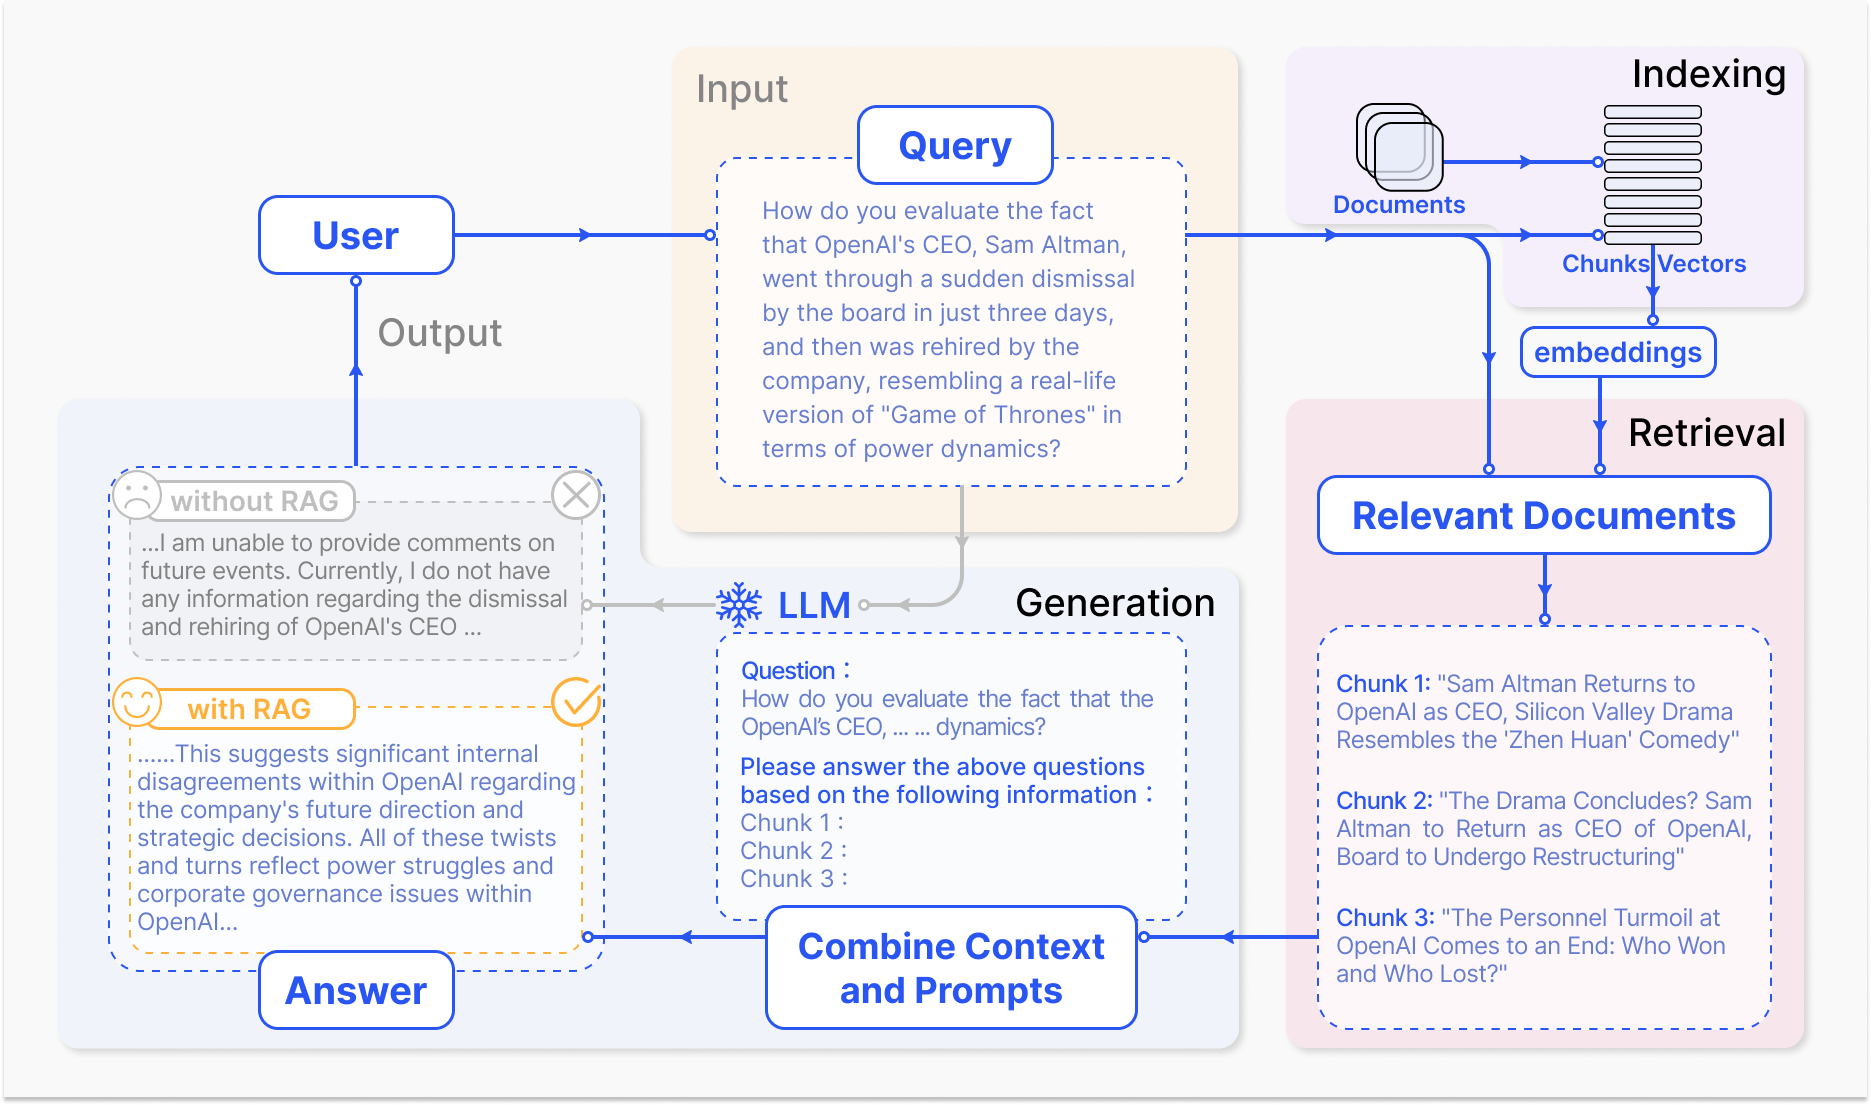
\includegraphics[width=\textwidth]{media/RAG_case.png}
    \caption{%
    Fluxo de informações com \textit{Retrieval-Augmented Generation} (RAG) e sem RAG em um LLM\@.
    Fonte:~\cite{gao2023retrieval}.\label{fig:rag_case}}
\end{figure*}

A \cref{fig:rag_case} apresenta um exemplo de aplicação do RAG no ChatGPT dada uma \textit{query} (busca, pergunta) que obriga o modelo a buscar informações relevantes em documentos externos pois a informação não está presente em seu conjunto de treinamento.
De modo geral, RAG é dividido em três etapas: indexação, recuperação e geração.
Detalhadamente, o RAG segue o seguinte fluxo: (1) indexar documentos relevantes e transformá-los em vetores de contexto; (2) recuperar os $k$-melhores vetores para uma dada consulta; (3) concatenar os vetores de contexto recuperados com a entrada e repassar ao LLM~\cite{gao2023retrieval}.

\noindent\textbf{Indexação (\textit{indexing})}: documentos relevantes em diversos formatos são ``lidos'', processados e transformados em vetores de contexto.
Documentos podem ser textos, PDFs, imagens, áudios, e afins.
Aqui, ``lidos'' significa que de alguma forma o conteúdo do documento é convertido em um formato que o sistema de armazenamento vetorial possa entender e processar --- por exemplo, um arquivo em PDF é convertido em texto puro e suas imagens são extraídas e transformadas em texto --- e então é transformado em um vetor de contexto.
Os detalhes de como essa transformação é feita dependem do tipo de documento e do sistema de armazenamento vetorial utilizado e não fazem parte do escopo desse trabalho.

\noindent\textbf{Recuperação (\textit{retrieval})}: dado um vetor de consulta, o banco de dados vetorial retorna os $k$-melhores vetores que mais se assemelham ao vetor de consulta.
A busca pode ser feita utilizando funções heurísticas, buscas hierárquicas ou outras técnicas.
Cabe ao implementador decidir qual a melhor função de busca para um determinado conjunto de documentos e seus vetores.

\noindent\textbf{Geração (\textit{generation})}: os vetores de contexto recuperados são concatenados com a entrada e repassados ao LLM para geração de uma resposta enriquecida com o contexto recuperado.

Existem três tipos de RAG\@: \textit{naïve}, \textit{advanced} (avançado) e modular.
\textit{Naïve} RAG é o mais simples e consiste apenas em indexação, recuperação e geração.
Esse tipo de RAG pode trazer problemas na qualidade das respostas geradas pois o modelo pode simplesmente repetir o conteúdo recuperado sem entender o contexto e sem adicionar informações.
\textit{Advanced} RAG é uma evolução do \textit{naïve} RAG que implementa estratégias de pré-recuperação e pós-recuperação para melhorar a qualidade dos vetores de contexto recuperados, além de aplicar técnicas de janela deslizante para melhorar a indexação.
Por fim, RAG modular é uma abordagem mais complexa que divide o processo de RAG em módulos independentes, onde cada módulo é responsável por uma etapa do processo, incorporando diversas estratégias para melhorar o desempenho do sistema como um todo.
A \cref{fig:rag_naive_advanced} apresenta uma comparação entre RAG \textit{naïve} e avançado, 
onde é possível observar que o \textit{advanced} RAG possui estratégias de pré-recuperação e pós-recuperação para melhorar a qualidade dos vetores de contexto recuperados.
A \cref{fig:rag_modular} apresenta a arquitetura de um RAG modular, onde o processo de RAG é dividido em módulos independentes, cada um responsável por uma etapa do processo.
Um RAG modular pode incorporar RAG \textit{naïve} e avançado, além de outras estratégias para melhorar o desempenho do sistema como um todo~\cite{lewis2020retrieval,gao2023retrieval}.

\begin{figure}[h]
    \centering
    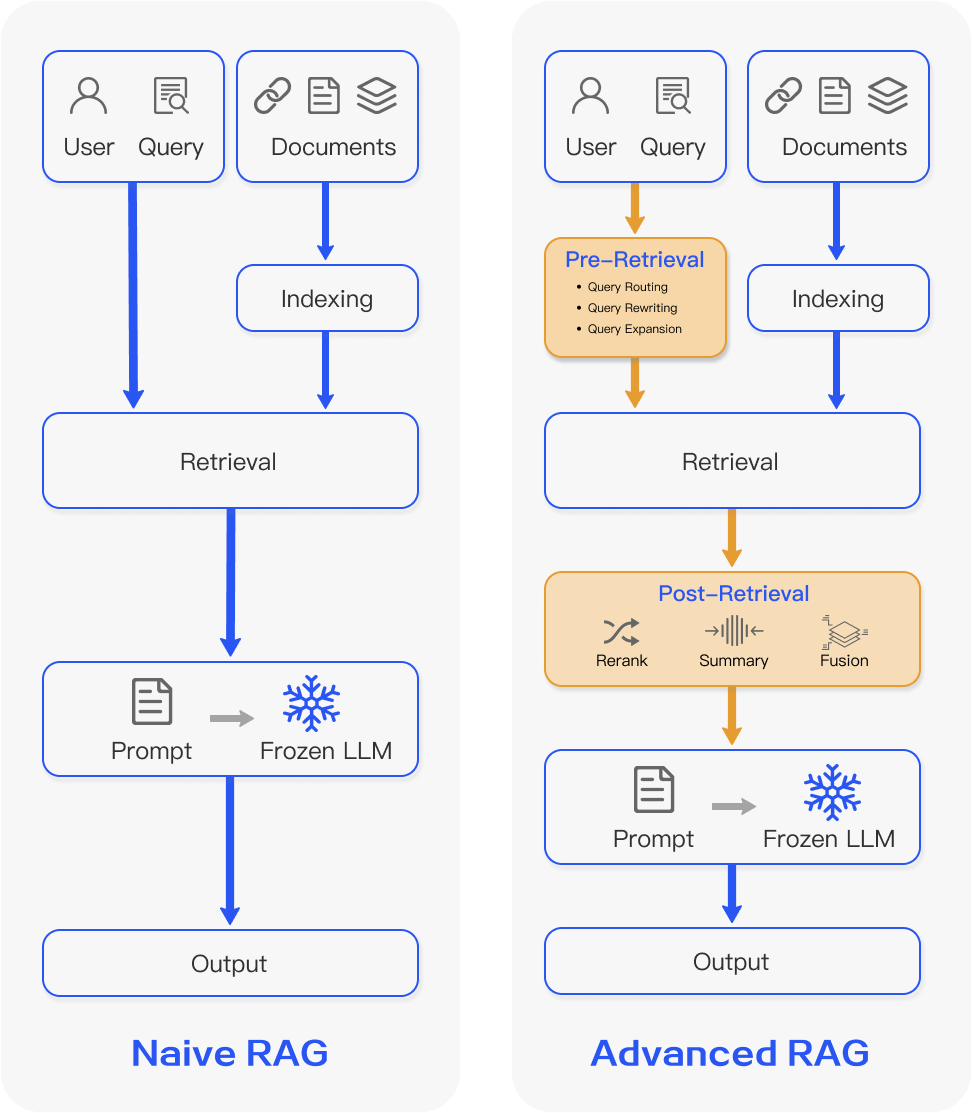
\includegraphics[width=\columnwidth]{media/RAG_naive_advanced.png}
    \caption{%
    Comparação entre \textit{naïve} e \textit{advanced} RAG\@.
    Fonte:~\cite{gao2023retrieval}.\label{fig:rag_naive_advanced}}
\end{figure}

\begin{figure}[h]
    \centering
    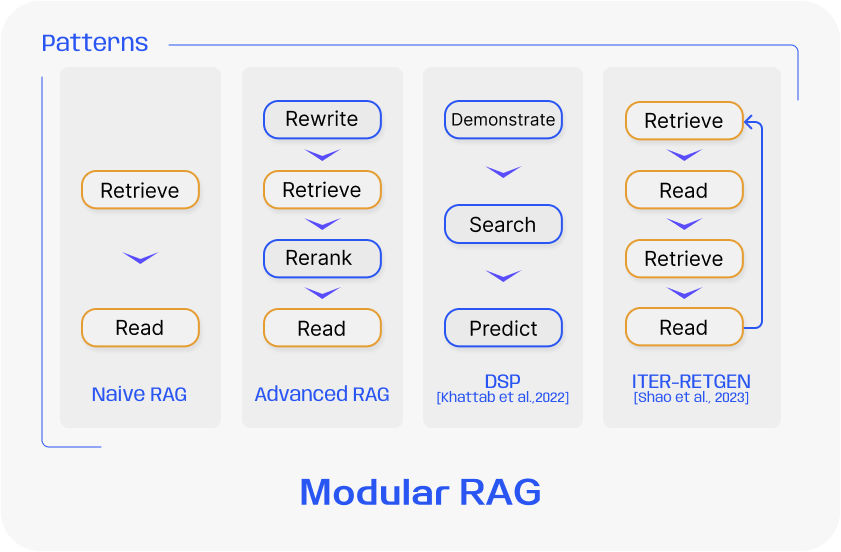
\includegraphics[width=0.9\columnwidth]{media/RAG_modular.png}
    \caption{%
    Arquitetura de um RAG modular.
    Fonte:~\cite{gao2023retrieval}.\label{fig:rag_modular}}
\end{figure}

Outra alternativa para introduzir conhecimento de um domínio previamente desconhecido a um LLM é a utilização de \textit{fine-tuning} e \textit{transfer learning}, onde o modelo é treinado em um conjunto de dados específico para uma tarefa específica~\cite{vaswani2017attention,devlin2018bert}.
Entre RAG e \textit{fine-tuning}, RAG é uma técnica mais flexível e que não requer um conjunto de dados de treinamento específico, pois o conhecimento é extraído de documentos externos de maneira dinâmica~\cite{lewis2020retrieval}, enquanto \textit{fine-tuning} requer um conjunto de dados de treinamento específico para a tarefa desejada e cria um novo modelo, o que pode ser problemático em um uso onde os documentos relevantes estão sempre mudando.

\subsection{\textit{Prompt-based tuning} em LLMs}

\noindent%
Um estudo recente apresenta um novo paradigma para especialização de LLMs modernos, \textit{prompt-based tuning}, ao invés de \textit{fine-tuning}~\cite{liu2023pre}.
Em seu estudo, os autores apresentam esse paradigma e o comparam com o anterior, o \textit{pre-train, fine-tune}, que consiste em treinar um LLM em um grande conjunto de dados e então ajustar os pesos do modelo para uma tarefa específica.
Esse novo paradigma consiste em escrever \textit{prompts} detalhados para resolver uma tarefa específica sem a necessidade de adaptar um LLM para isso.
Por exemplo, é possível fazer análise de sentimentos utilizando o modelo com a seguinte \textit{prompt}: ``Complete the phrase: `I missed the bus today, I felt so \_'\,'', onde o modelo completaria a frase com uma palavra que expressa um sentimento, como ``disappointed''~\cite{liu2023pre}.
Os estudos~\cite{wei2022finetunedlanguagemodelszeroshot,kong2023better} apresentam abordagens similares, com resultados alinhados ao apresentado em~\cite{liu2023pre}.

Dito isso, \textit{prompt-based tuning} introduz a necessidade de realizar uma engenharia de \textit{prompts}, também conhecido como \textit{prompt engineering}, para obter um resultado efetivo ao questionar o modelo.

\section{Trabalhos relacionados e revisão da literatura\label{sec:trab_rel}}

\noindent%
Nos últimos anos, houve um avanço significativo no desenvolvimento e aplicação de LLMs,
que evoluíram desde modelos de linguagem estatísticos até redes neurais, culminando na era atual de GPTs muito poderosos.
Revisões abrangentes feitas em~\cite{bommasani2021opportunities} e~\cite{zhao2023survey} fornecem uma análise aprofundada desses desenvolvimentos, destacando a evolução desde métodos estatísticos até redes neurais e os avanços subsequentes com GPTs e LLMs.
Nelas são abordados aspectos do pré-treinamento, adaptação, utilização e avaliação de capacidade, o que oferece uma visão detalhada do estado-da-arte na pesquisa de LLMs.
Os autores apontam que LLMs como BERT, GPT-4, LLaMA, ChatGPT e Claude não apenas melhoraram o desempenho de várias tarefas de PLN, mas também abriram caminho para novas aplicações de IA, transformando significativamente o campo.

A seguir é apresentada uma revisão dos trabalhos relacionados, que abordam o uso de modelos de linguagem na aprendizagem e aprendizagem e o desenvolvimento de metodologias para a aprendizagem de programação.

\subsection{Large language models in education: A focus on the complementary relationship between human teachers and ChatGPT (2023)}
\noindent%
O trabalho de~\cite{jeon2023large} explora o uso de modelos de linguagem na aprendizagem, com foco na relação complementar entre professores humanos e ChatGPT na aprendizagem de inglês para estrangeiros na Coreia do Sul.
Nele, os autores examinam como o ChatGPT pode complementar os papéis dos professores humanos, onde identificaram que o ChatGPT assume quatro papéis principais: interlocutor, gerador de conteúdo, assistente de aprendizagem e avaliador.
Além disso, os autores discutem o papel dos professores em conscientizar os estudantes sobre o uso de ferramentas como o ChatGPT e como eles podem ser usados para melhorar o aprendizado.
O trabalho destaca a importância de professores e modelos de linguagem trabalharem juntos para melhorar o aprendizado dos estudantes, e confirma que \ul{professores necessitam de treinamento para utilizar ferramentas de IA em sala de aula}~\cite{jeon2023large,celik2022promises}.

\subsection{ChatGPT for good? On opportunities and challenges of large language models for education (2023)}
\noindent%
O trabalho de~\cite{kasneci2023chatgpt} investiga as oportunidades e desafios do uso de LLMs, como ChatGPT, na aprendizagem.
Os autores discutem como esses modelos podem ser utilizados em diferentes contextos educacionais e momentos de desenvolvimento (infância, adolescência, idade adulta), e como eles podem ser utilizados para melhorar o engajamento dos discentes e personalizar suas experiências.
Além disso, discutem a \ul{necessidade de desenvolver competências entre professores e alunos para entender e utilizar essas tecnologias de maneira eficaz}, ressaltando a importância do pensamento crítico e estratégias de verificação de fatos.
O estudo também aborda questões éticas, como o viés potencial nas respostas geradas e a necessidade de supervisão humana contínua, e oferece recomendações para uma integração responsável e ética desses modelos no ambiente educacional~\cite{kasneci2023chatgpt}.

\subsection{ChatGPT no auxílio da aprendizagem de programação: um estudo de caso (2023)}
\noindent%
O estudo de~\cite{da2023chatgpt} investiga o uso do ChatGPT como ferramenta auxiliar na aprendizagem de programação.
Utilizando uma metodologia quali-quantitativa, os autores analisaram como o ChatGPT pode apoiar os alunos na compreensão de conceitos, fornecendo exemplos de código e feedback personalizado.
Os resultados indicam que, embora o ChatGPT seja uma tecnologia promissora para a aprendizagem da programação, ele apresenta limitações, como a precisão das respostas e a necessidade de orientação contínua por parte dos professores para evitar mal-entendidos.
O estudo destaca a importância de integrar tecnologias de IA de forma cuidadosa e monitorada para melhorar o aprendizado e o engajamento dos alunos~\cite{da2023chatgpt}.

\subsection{Ensino de Programação Orientada a Objetos Para Iniciantes: Uma Metodologia para Programação Criativa (2023)}
\noindent%
O artigo de~\cite{giraffa2023ensino} explora metodologias para a aprendizagem de programação orientada a objetos (POO) a iniciantes, especialmente no contexto de ensino remoto durante a pandemia.
A metodologia aplicada incluiu a utilização de salas de aula invertidas, metodologias ativas, e integração de projetos práticos, com o objetivo de desenvolver o pensamento computacional dos alunos.
Os resultados destacaram tanto as oportunidades quanto os desafios enfrentados, como restrições tecnológicas e a necessidade de supervisão constante.
Segundo~\cite{giraffa2023ensino}, os estudantes valorizaram a experiência remota, destacando a qualidade dos conteúdos e dos trabalhos práticos.
O estudo enfatiza a importância de futuras pesquisas sobre estratégias de aprendizagem de programação, considerando a proposta metodológica de Programação Criativa como uma abordagem eficaz para promover a aprendizagem integral e o desenvolvimento de habilidades essenciais na área de programação.
Também é enfatizado por~\cite{giraffa2023ensino} a importância de desenvolver o Pensamento Computacional (PC)~\cite{wing2008computational} nos alunos, e como a metodologia de Programação Criativa pode ser uma abordagem eficaz para desenvolver essas habilidades.

\subsection{Can artificial intelligence transform higher education? (2020)}
\noindent%
O artigo de~\cite{bates2020can} explora o impacto potencial e real da IA no ensino superior.
Os autores examinam diversas aplicações de IA, como sistemas tutores inteligentes, análise de aprendizado e personalização adaptativa.
Apesar do potencial significativo da IA para transformar práticas de aprendizagem, os resultados empíricos atuais mostram que a influência da IA na melhoria de resultados de aprendizagem ainda é marginal.
Os autores destacam a necessidade de maior envolvimento dos educadores no desenvolvimento de IA educacional para garantir que as aplicações futuras abordem habilidades críticas e pensamento criativo~\cite{bates2020can}.
Vale ressaltar que o trabalho de~\cite{bates2020can} foi publicado em 2020, e desde então novos avanços e pesquisas em IA educacional, além de novos modelos mais poderosos e coerentes, têm sido realizados, o que pode impactar as conclusões apresentadas no artigo.

\subsection{Análise dos trabalhos estudados}

\noindent%
É possível observar que a utilização de modelos de linguagem na aprendizagem é uma tendência ascendente, com diversos estudos explorando como esses modelos podem ser utilizados para melhorar o aprendizado dos estudantes.
Os trabalhos de~\cite{jeon2023large,kasneci2023chatgpt,da2023chatgpt} destacam a importância de professores e IA trabalharem juntos para melhorar o aprendizado dos estudantes, e ressaltam a necessidade de treinamento e supervisão contínua para garantir o uso ético e responsável dessas tecnologias.
Já o trabalho de~\cite{giraffa2023ensino} explora metodologias para a aprendizagem de programação orientada a objetos a iniciantes, destacando a importância do pensamento computacional dos alunos e como a aprendizagem de programação não é apenas sobre a linguagem de programação, mas sobre o desenvolvimento de outras habilidades essenciais na área de computação.
Por fim, o trabalho de~\cite{bates2020can} examina o impacto potencial e real da IA no ensino superior, destacando o potencial significativo da IA para transformar práticas de aprendizagem.
Esses trabalhos contribuem para a compreensão de como a IA pode ser utilizada para melhorar o aprendizado dos estudantes e como professores e IA podem trabalhar juntos para alcançar esse objetivo.
Em vista disso, este trabalho busca contribuir para essa discussão, explorando como um sistema de IA pode ser utilizado para auxiliar discentes na aprendizagem de programação, fornecendo respostas personalizadas e orientações para suas dúvidas, além de agregar valor à instituição que o adotar.

\subsection{Conexões com o trabalho desenvolvido}

\noindent%
A integração da IA no aprendizado e processos de aprendizagem tem sido amplamente estudada, com diversas abordagens demonstrando os potenciais benefícios e desafios do uso da IA para melhorar as experiências de aprendizado.
Por exemplo,~\cite{jeon2023large} explora a relação complementar entre professores humanos e o ChatGPT na aprendizagem de inglês, enfatizando a necessidade de os professores incorporarem efetivamente ferramentas de IA em suas estratégias de aprendizagem~\cite{jeon2023large}.
Este estudo fornece uma base para entender como a IA pode apoiar os educadores, um conceito examinado por este trabalho ao aplicar IA Generativa na aprendizagem de programação.

De modo similar,~\cite{kasneci2023chatgpt} discute as oportunidades e desafios do uso de grandes modelos de linguagem, como o ChatGPT, em vários contextos do aprendizado, destacando a importância das competências de professores e alunos na utilização dessas tecnologias~\cite{kasneci2023chatgpt}.
Este estudo aborda um assunto similar, focado especificamente no domínio da aprendizagem de programação e propondo implementações práticas para apoiar tanto os alunos quanto as instituições de ensino durante sua trajetória acadêmica.

A pesquisa de~\cite{da2023chatgpt} sobre o uso do ChatGPT para auxiliar a aprendizagem de programação destacou tanto o potencial quanto as limitações desse modelo em fornecer feedback personalizado e exemplos de código~\cite{da2023chatgpt}.
Isso se alinha com o objetivo de utilizar um LLM para oferecer suporte personalizado aos alunos, abordando limitações semelhantes por meio de capacidades avançadas do modelo e implantação estruturada em ambientes educacionais.

As taxas de reprovação em cursos introdutórios de programação foram revisitadas por~\cite{watson2014failure}, atribuindo a alta evasão à complexidade dos conceitos e à falta de suporte~\cite{watson2014failure}.
Abordando essa lacuna, este estudo visa reduzir as taxas de evasão ao fornecer assistência em tempo real gerada por IA para ajudar os alunos a superar obstáculos de aprendizagem.

No entanto, nenhum desses estudos integra diretamente o material didático do curso, como é feito nesse trabalho.
Este estudo se destaca por utilizar a IA Generativa para fornecer respostas e orientações baseadas no material específico das disciplinas, criando um ambiente de aprendizagem altamente personalizado e contextualizado.
Os trabalhos apresentados anteriormente foram escolhidos por tangenciarem ao menos um dos temas abordados nesse trabalho, como a importância da integração de IA no aprendizado, a necessidade de treinamento e supervisão contínua para garantir o uso ético e responsável dessas tecnologias, e a importância do pensamento computacional e do desenvolvimento de habilidades essenciais na área de computação.

Ao se basear nesses estudos fundamentais, essa pesquisa visa contribuir para a área de IA na aprendizagem, focando em sua aplicação em cursos de programação.
O sistema implementado e sua integração nos \textit{frameworks} educacionais busca não apenas validar a eficácia da IA em melhorar os resultados de aprendizagem, mas também oferecer uma solução escalável para os desafios generalizados na aprendizagem da Ciência da Computação.

\section{Trabalho desenvolvido\label{sec:desenvolvimento}}

\noindent%
Neste trabalho é apresentado um sistema de apoio ao aprendizado de programação utilizando modelos de linguagem de grande escala capazes de responder perguntas dos estudantes e fornecerem orientações personalizadas baseando-se em materiais didáticos de determinada disciplina.
O sistema desenvolvido fora arquitetado para ser modificável e expansível, permitindo a adição de novas funcionalidades, outros modelos, outras interfaces, outros sistemas de RAG, e até mesmo a integração com outras ferramentas de aprendizagem.
Dito isso, o escopo do trabalho se limita às ferramentas Ollama para execução do modelo, OpenWebUI como interface web, e Pipelines com LlamaIndex como sistema de RAG\@.
O sistema possui os seguintes requisitos básicos:

\begin{itemize}
    \item Responder perguntas utilizando informações externas à seu treinamento através de extensão de conhecimento.
    \item Evitar dar respostas diretas, tentando aplicar técnicas de aprendizagem guiada.
    \item Dar respostas coesas e corretas seguindo o material didático.
    \item Não diminuir a capacidade de inferência do modelo-base.
    \item Ser de fácil uso e acesso; acesso se dá, por exemplo, por uma interface web.
    \item Agregar valor tanto ao aprendizado do discente quanto ao trabalho do docente.
\end{itemize}

As seções seguintes contextualizam o problema abordado e detalham a implementação do sistema.

\subsection{Pensamento computacional e evasão em cursos de computação}

\noindent%
A evasão nos cursos de computação é um problema recorrente e preocupante, tanto no Brasil quanto no exterior~\cite{alvim2024evasao,takacs2022,kinnunen2006students,hoed2017analise,watson2014failure}.
Diversos fatores contribuem para esse fenômeno, entre eles a dificuldade de aprendizagem dos conceitos fundamentais de programação e lógica~\cite{takacs2022,giraffa2023ensino}.
Essas dificuldades são amplamente atribuídas à falta de familiaridade dos alunos com o pensamento computacional~\cite{wing2008computational}, uma habilidade essencial que vai além do simples domínio de uma linguagem de programação~\cite{oliveira_de_souza_2022,hong2020introduction,gomes2017desenvolvendo,de2024ensino}.

O pensamento computacional envolve a capacidade de resolver problemas de maneira lógica e estruturada, habilidades cruciais para o sucesso em qualquer área da computação e outras áreas do conhecimento~\cite{wing2008computational}.
No entanto, muitos alunos encontram barreiras significativas ao tentar desenvolver essas habilidades, o que pode levar à frustração e, eventualmente, à desistência do curso ou até mesmo da área.
Os estudos de~\cite{hoed2017analise,kinnunen2006students,watson2014failure} apontam que a evasão em cursos de computação é um problema complexo, influenciado por diversos fatores, sendo apenas um deles a dificuldade de aprendizagem desses conceitos.
Dito isso, uma ferramenta que auxilie o professor e o discente na aprendizagem desses conceitos é de grande valia.

\subsection{IA no apoio ao aprendizado}

\noindent%
A aplicação da IA no apoio ao aprendizado não é uma novidade, mas suas possibilidades estão se expandindo rapidamente~\cite{bates2020can}.
Embora uma revisão sistemática de pesquisas sobre aplicações de IA no ensino superior sugira que a integração efetiva de IA pode melhorar os resultados de aprendizagem ao fornecer suporte personalizado e adaptativo aos estudantes~\cite{zawacki2019systematic},~\cite{bates2020can} apresenta um cenário mais complexo, onde seus resultados mostram que a influência da IA obtém melhorias marginais.
Reforça-se que o papel dos educadores é crucial para a implementação bem-sucedida dessas tecnologias~\cite{oliveira_de_souza_2022,kasneci2023chatgpt,jeon2023large}.

O pensamento computacional é fundamental para o sucesso dos alunos não só em cursos de computação mas em diversas outras áreas que possivelmente nem existam ainda~\cite{wing2008computational,wef2019schools}.
Diversas estratégias podem ser empregadas para ensinar essas habilidades em diferentes contextos e ambientes de aprendizagem.
Se cita:

\noindent\textbf{Integração de conceitos computacionais no currículo}:
Estudos mostram que incorporar conceitos computacionais no currículo do ensino fundamental e médio pode ajudar a desenvolver habilidades de pensamento computacional em estudantes de todas as idades~\cite{oliveira_de_souza_2022,hong2020introduction,gomes2017desenvolvendo,de2024ensino}.

\noindent\textbf{Aprendizagem baseada em projetos}:
Projetos práticos que envolvem a criação de programas ou a resolução de problemas complexos incentivam os alunos a aplicar o pensamento computacional de forma criativa e prática.
Este método não apenas reforça os conceitos aprendidos, mas também promove habilidades de colaboração e comunicação~\cite{hong2020introduction,wef2019schools,giraffa2023ensino,oliveira_de_souza_2022}.

\noindent\textbf{Feedback e avaliação contínua}:
O uso de sistemas de avaliação contínua e feedback imediato pode ajudar os alunos a identificar suas dificuldades e melhorar suas habilidades de pensamento computacional ao longo do curso.
A integração com sistemas de IA pode fornecer suporte personalizado e orientações específicas para cada aluno dadas suas necessidades e dificuldades~\cite{jeon2023large,kasneci2023chatgpt,da2023chatgpt}.
Nesse sentido também é possível citar a importância de ferramentas de apoio à aprendizagem, como o sistema desenvolvido neste trabalho, que podem fornecer dados valiosos para análise de aprendizado (\textit{learning analytics}) e ajudar a identificar padrões e tendências no desempenho dos alunos~\cite{jeon2023large,bates2020can}.

\noindent\textbf{Treinamento de educadores}:
A eficácia da aprendizagem de pensamento computacional também depende da preparação dos educadores.
Oferecer treinamento adequado para professores é crucial para que eles possam integrar essas estratégias em suas aulas de maneira eficaz~\cite{kasneci2023chatgpt,jeon2023large}.

Empregar IA na aprendizagem também se faz atraente pois pode fornecer suporte personalizado e adaptativo aos estudantes, ajudando a superar obstáculos de aprendizagem de maneira individual e sem julgamentos~\cite{zawacki2019systematic,guzdial2015learner}.

\subsection{Escolha do modelo de IA}

\noindent%
Existem muitos LLMs disponíveis, cada um com suas características e limitações~\cite{radford2019language,zhao2023survey}.
Para manter o estudo alinhado com o mercado e não correr tanto risco de expor os usuários a modelos inseguros, foram considerados apenas aqueles vindos de empresas de renome (Google, Microsoft, Meta, \textit{etc.}) com ampla documentação e abordagens éticas e de segurança bem definidas.
Desses, foram descartados modelos de código-fechado como toda a família de modelos da OpenAI\@: GPT-3~\cite{floridi2020gpt}, GPT-4, ChatGPT, entre outros.
Entre os modelos de \textit{open source} (código aberto), a família de modelos LLaMA se destacou por sua performance excelente em diversos \textit{benchmarks} (testes padronizados) e se tornou muito popular na indústria e pesquisa~\cite{zhao2023survey,touvron2023llama,touvron2023llama2}.
No início dessa pesquisa, o modelo LLaMA 3 ainda não havia sido lançado; mesmo assim, a família LLaMA já havia sido escolhida como a melhor opção para o desenvolvimento do sistema desenvolvido~\cite{zhao2023survey,touvron2023llama,touvron2023llama2}.
Com o lançamento do LLaMA 3, a escolha foi confirmada, e essa família foi escolhida~\cite{meta2024llama3,llama3modelcard}.
Outros motivos que reforçam nossa escolha dessa família são sua documentação extensa e, de muita importância, a ênfase que a equipe de desenvolvimento dá à ética e segurança em seus modelos~\cite{meta2024llama3,llama3modelcard,inan2023llama}.

Não se levou em consideração apenas os resultados das \textit{benchmarks} auto-reportados pelas equipes de desenvolvimento de cada modelo.
Como já haviam sido descartados modelos de código fechado, a utilização dos resultados de \textit{benchmarks} de terceiros se tornou possível, especialmente os realizados por~\cite{zhao2023survey}, o Open LLM Leaderboard~\cite{open-llm-leaderboard} da HuggingFace e o AlpacaEval 2.0~\cite{alpaca_eval}.
Também foram removidas as versões quantizadas, modificadas ou com \textit{fine-tuning} da busca, mas foram mantidos aqueles modelos modificados (\textit{fine-tuned}) para tarefas específicas como \textit{chat} e código.

\subsubsection{Open LLM Leaderboard}

\noindent%
O Open LLM Leaderboard é uma plataforma que automaticamente avalia modelos abertos utilizando técnicas conhecidas de avaliação como ARC~\cite{clark2018think}, HellaSwag~\cite{zellers2019hellaswag}, MMLU~\cite{hendrycks2021measuring} e WINOGRANDE~\cite{DBLP:journals/corr/abs-1907-10641}.
Também utilizam métricas para avaliar conhecimentos em áreas específicas como matemática (GSM8K~\cite{DBLP:journals/corr/abs-2110-14168}) e falácias (TruthfulQA~\cite{lin2022truthfulqa}).
Como o Open LLM Leaderboard avalia muitos modelos diferentes, foi utilizado um filtro para remover aqueles que são previamente treinados em tarefas específicas (\textit{fine-tuned on domain-specific datasets}, em inglês) e mantidos apenas modelos pré-treinados para que a comparação fosse justa e os resultados refletissem a capacidade dos modelos de aprender e generalizar conhecimento~\cite{open-llm-leaderboard}.
No Open LLM Leaderboard, o LLaMA 3 70B se coloca em primeiro lugar na média, com um escore de $73.96$.
Seguido em perto por Qwen 72B com um escore médio de $73.6$ e uma versão modificada do Phi 3 com um escore de $73.57$.
Outros modelos considerados foram o Deepseek 67B (escore de $69.38$) e o Mixtral 8x7B (escore de $68.42$).

\subsubsection{AlpacaEval 2.0}

\noindent%
O AlpacaEval 2.0 é uma plataforma de avaliação de modelos de linguagem automática que utiliza um conjunto de avaliação própio e aberto que avalia LLMs entre si, comparando suas respostas com as respotas geradas pelo OpenAI GPT-4 Preview; o escore é chamado de \textit{win rate}, ou taxa de vitória~\cite{alpaca_eval}.
Quando comparado com o Open LLM Leaderboard, o AlpacaEval 2.0 é mais focado em avaliar a capacidade dos modelos entre si, enquanto o Open LLM Leaderboard é mais abrangente e avalia uma variedade de tarefas~\cite{alpaca_eval,open-llm-leaderboard}.
No AlpacaEval 2.0, o LLaMA 3 70B se coloca décimo lugar com uma taxa de vitórias de $34.4\%$.
Os modelos que se colocam acima do LLaMA sâo o OpenAI GPT-4 e suas variações, 01.AI Yi Large, Anthropic Claude 3 Opus e Qwen 1.5 72B.
Como um dos requisitos é utilizar modelos de código aberto, foram descartadas as famílias OpenAI GPT-4 e Anthropic Claude 3.
Entre os modelos restantes, o LLaMA 3 70B se destaca por possuir ampla documentação, fundamentação científica e ênfase em segurança e ética~\cite{meta2024llama3,llama3modelcard}.

\subsection{LLaMA 3\label{sec:llama3}}

\noindent%
A família de modelos escolhida foi a Meta LLaMA 3, sucessora da LLaMA 2 e Codellama.
Dentro da família LLaMA 3 existem dois modelos-base ou fundamentais: \texttt{llama3:8b} e \texttt{llama3:70b}, que se diferenciam pela quantidade de parâmetros e, consequentemente, pela capacidade de processamento e requisitos computacionais~\cite{meta2024llama3,llama3modelcard}.
O modelo \texttt{llama3:8b} possui oito bilhões de parâmetros e é menor e mais rápido, enquanto o \texttt{llama3:70b} é maior, com setenta bilhões de parâmetros, e mais poderoso, mas também mais exigente em termos de recursos computacionais~\cite{meta2024llama3}.
Existe também o \texttt{llama3:400b}, com quatrocentos bilhões de parâmetros e quase seis vezes maior que o \texttt{llama3:70b}, que foi apenas anunciado e ainda não está disponível para uso~\cite{llama3_400b}.
As variações de número de parâmetros refletem diretamente na capacidade de processamento e na qualidade das respostas geradas pelo modelo, assim como em seus requisitos computacionais.
Para o uso em tarefas específicas, como \textit{chat} e código, são utilizadas as versões refinadas desses modelos, que são \textit{fine-tuned} para essas tarefas~\cite{meta2024llama3,llama3modelcard}.
A \cref{fig:metallama3eval} mostra uma comparação reportada pela Meta AI entre o LLaMA 3 70B Instruct e outros LLMs.

\begin{figure*}[ht!]
    \centering
    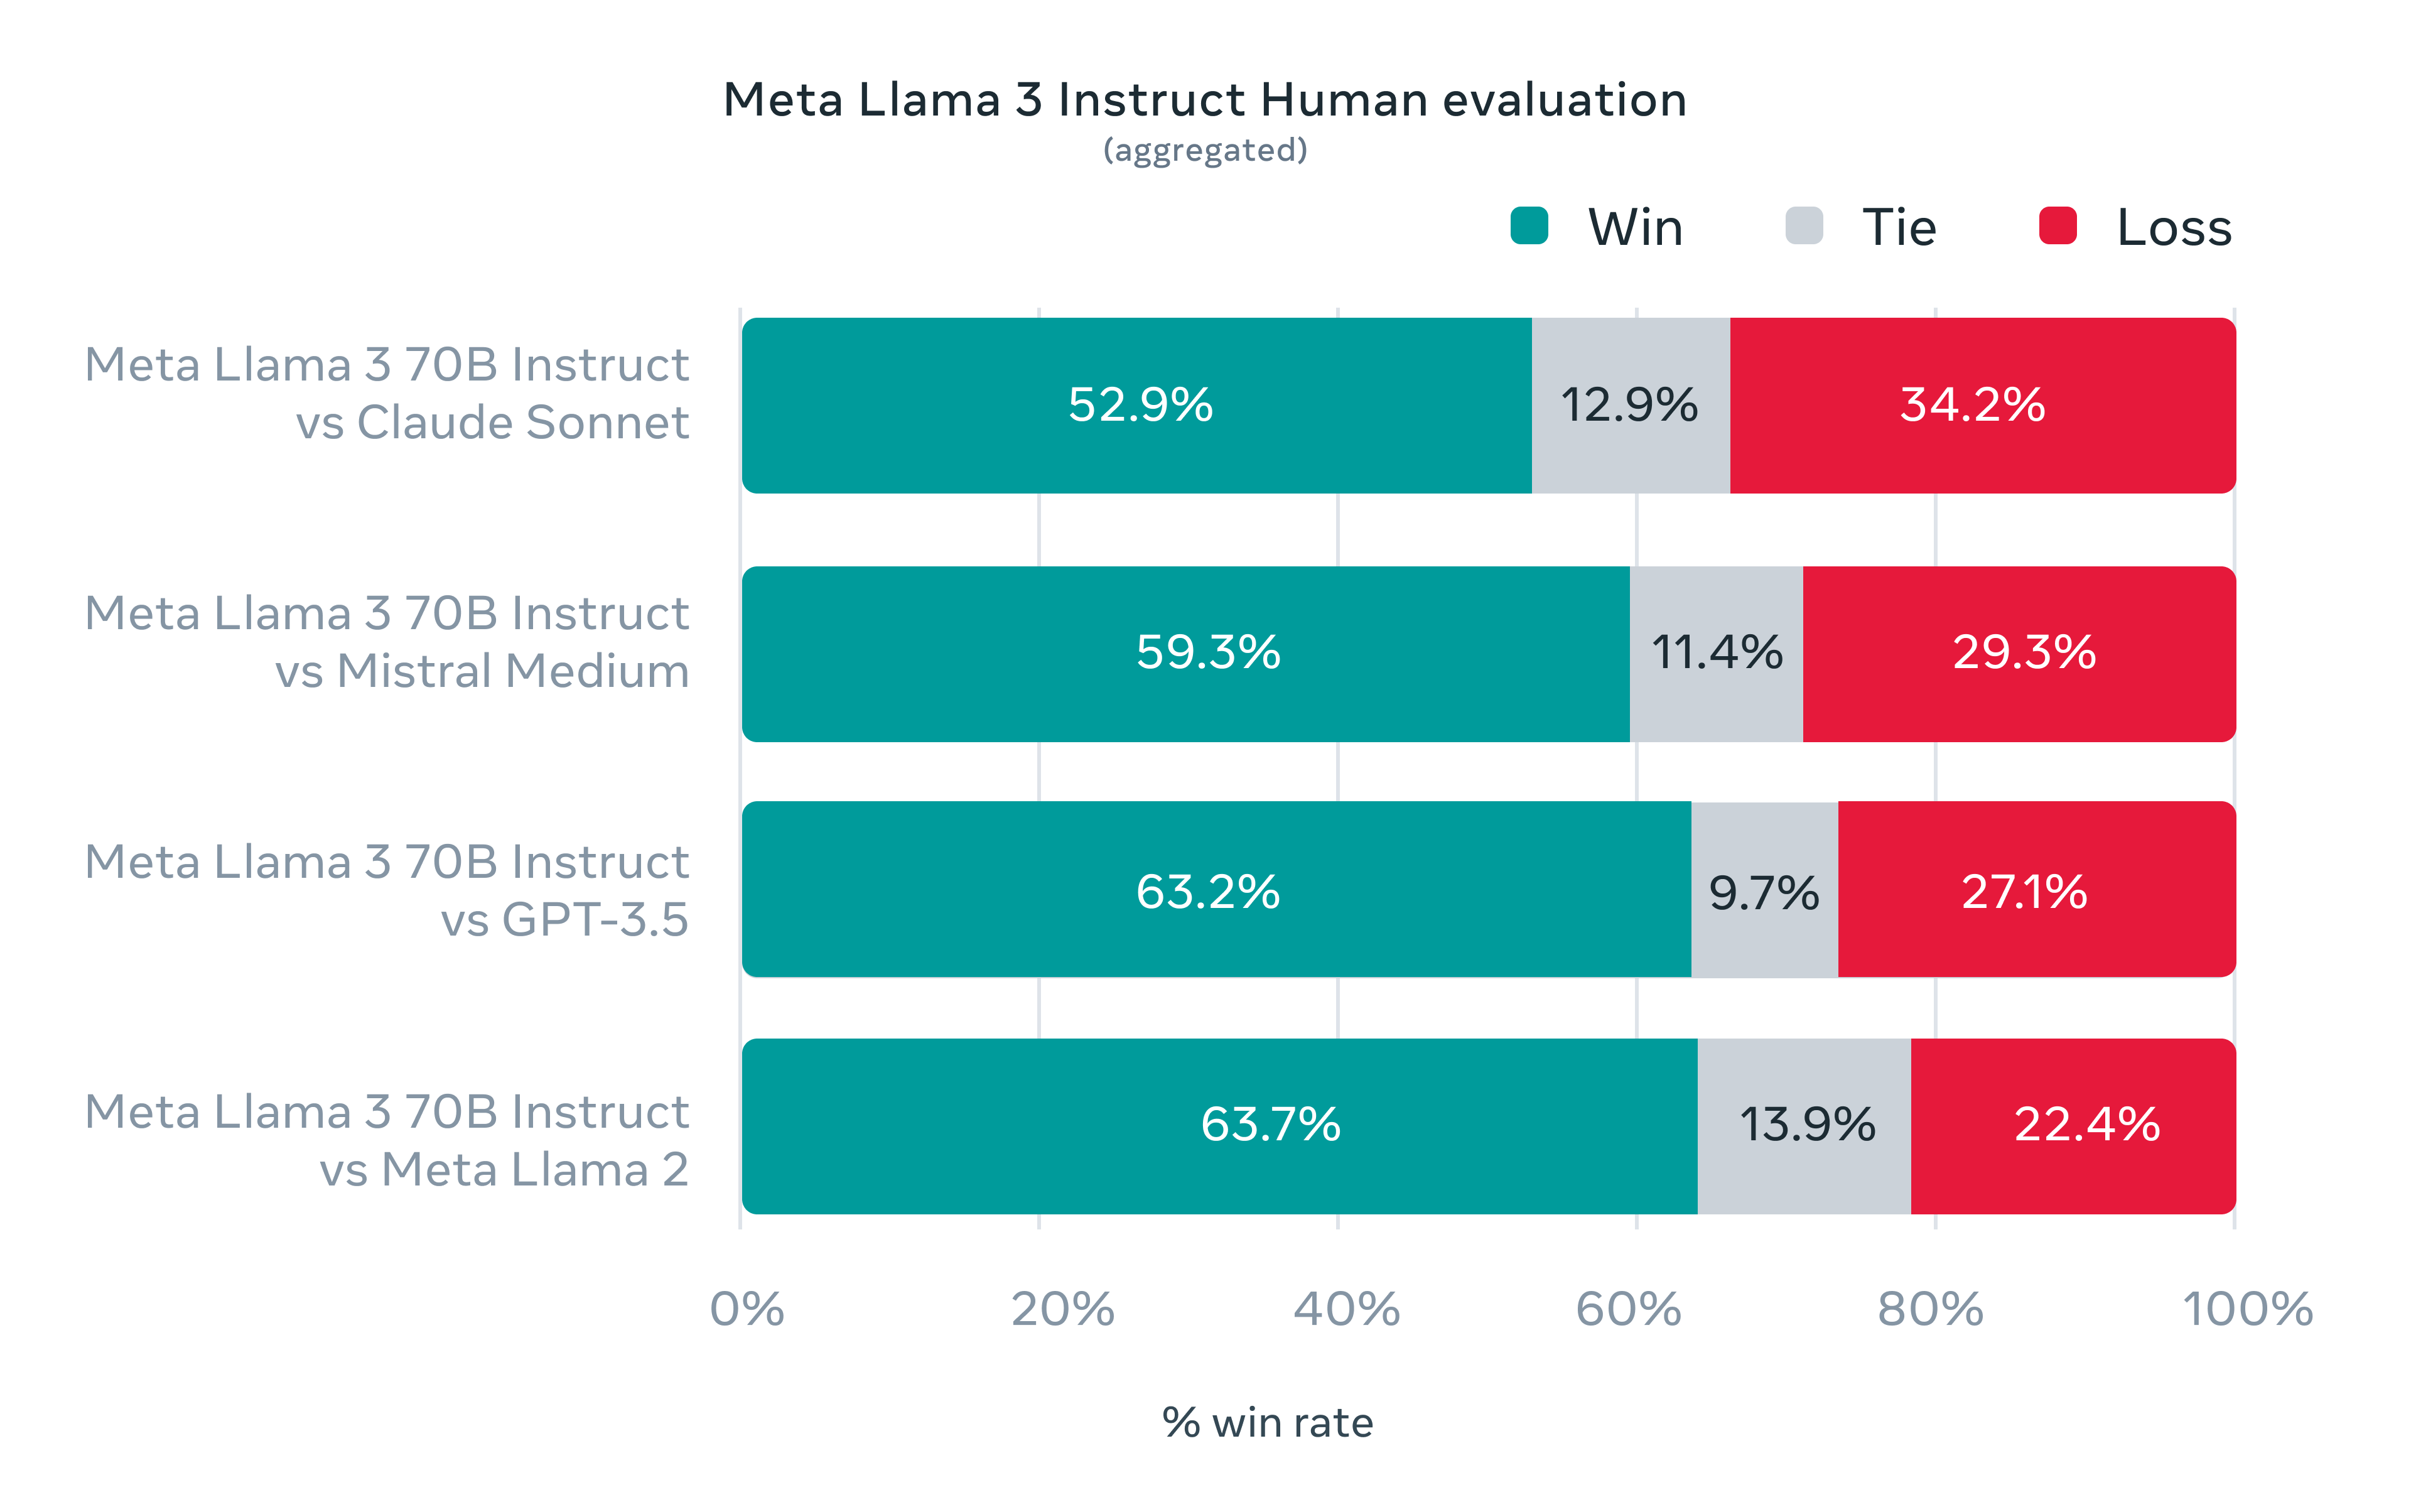
\includegraphics[width=\textwidth]{media/metallama3eval.png}
    \caption{Comparação reportada pela Meta AI entre o LLaMA 3 70B Instruct e outros LLMs. Fonte:~\cite{meta2024llama3}.\label{fig:metallama3eval}}
\end{figure*}

Para \textit{chats} e conversas há a variação \textit{instruct}, como o \texttt{llama3:70b-instruct}.
Diferente do LLaMA 2, o LLaMA 3 não possui uma variação específica para código, mas é possível utilizar o \texttt{llama3:70b-instruct} para essa tarefa~\cite{touvron2023llama2,meta2024llama3}.
Para código, não há um refinamento específico do LLaMA 3.
No entanto, existe o Codellama.
O Codellama é a versão \textit{fine-tuned} do LLaMA 2 para tarefas de código~\cite{roziere2023code}, e foi testado neste trabalho como uma alternativa aos modelos de conversação.

O LLaMA 3 possui conteúdos oficiais disponíveis em~\cite{meta2024llama3} e~\cite{llama3modelcard} que contém informações importantes sobre o modelo, como sua arquitetura e funcionamento.
Similar ao LLaMA 2, o LLaMA 3 utiliza \textit{grouped query attention} (GQA) como seu mecanismo de atenção.
No entanto, o LLaMA 3 aplica a GQA em ambos os tamanhos de modelo, enquanto o LLaMA 2 o aplica apenas nos modelos com 34 bilhões de parâmetros ou mais~\cite{meta2024llama3,touvron2023llama2}.
O \textit{tokenizer} do LLaMA 2 é o mesmo do LLaMA 1, com um vocabulário de 32 mil \textit{tokens}~\cite{touvron2023llama2}.
Já o \textit{tokenizer} do LLaMA 3 possui 128 mil \textit{tokens}, o que leva a uma melhoria substancial na performance de codificação (\textit{encoding})~\cite{meta2024llama3}.
Em sua arquitetura baixo nível, o LLaMA utiliza a função de ativação SwiGLU (\autoref{eq:fun_ativacao_swiglu}) e normaliza as saídas da rede antes de utilizar a função \textit{softmax} no resultado.

O \textit{dataset} de treinamento do LLaMA 3 é sete vezes maior que o do LLaMA 2, com mais de 15 trilhões de \textit{tokens}~\cite{meta2024llama3} e incluindo quatro vezes mais \textit{tokens} de código.
Desses 15 trilhões de \textit{tokens}, em torno de $5\%$ são de línguas diferentes do inglês, o que torna o LLaMA 3 um modelo multilíngue~\cite{meta2024llama3}.
Ou seja, mesmo que o modelo possa ser considerado multilíngue, não se espera que sua performance em outras línguas seja tão boa quanto em inglês.
Mesmo assim, nos testes conduzidos neste estudo, o LLaMA 3 se saiu bem em responder perguntas em português.

LLMs possuem um número máximo de \textit{tokens} que são considerados por vez durante a inferência.
Isso se chama tamanho ou janela de contexto, e varia de modelo a modelo.
O tamanho dessa janela determina quanto do texto anterior o modelo irá ``lembrar'', ou levar em consideração, ao gerar uma resposta coerente~\cite{vaswani2017attention,devlin2018bert,brown2020language}.

Ambos modelos (8B e 70B) possuem um tamanho máximo de contexto de 8 mil \textit{tokens}, mas é possível aumentar esse tamanho através de técnicas como LoRA e QLoRA, cujos conceitos não fazem parte do escopo deste trabalho.
Utilizando QLoRA,~\cite{zhang2024extending} reporta que foi possível aumentar o tamanho do contexto do LLaMA 3 8B Instruct para 80 mil \textit{tokens} com pouca perda de acurácia, e afirma que talvez seja possível aumentar o contexto ainda mais.

Segundo~\cite{meta2024llama3}, o treinamento dos modelos LLaMA 3 8B e 70B durou $1.3$ milhão e $6.4$ milhões de horas respectivamente em dois \textit{clusters} com 24 mil GPUs NVIDIA H100 com \SI{80}{\giga\byte} de VRAM cada.
Cada uma dessas GPUs é precificada em torno de 30 mil dólares americanos, e cada cluster possui $24.576$ GPUs, \ul{o que resulta em um custo apenas em GPUs, sem contar outros requisitos de infraestrutura, de quase um bilhão e meio de dólares americanos}~\cite{metagenaiinfra}.
Ou seja, o treinamento desses modelos é extremamente caro, exige uma infraestrutura computacional de ponta e recai sobre grandes empresas e instituições de pesquisa.

\subsubsection{Segurança}
Sobre segurança e ética,~\cite{inan2023llama} apresenta o Llama Guard, um LLM ``guardião'' capaz de detectar e corrigir viéses, discurso de ódio, desinformação, entre outros.
Em~\cite{meta2024llama3} é sugerido que o LLaMA 3 seja utilizado em conjunto com o Llama Guard para garantir a segurança e ética do sistema que será desenvolvido, onde o Llama Guard atua como um filtro de segurança tanto na entrada quanto na saída do sistema.
A segurança de LLMs é um fator importantíssimo a ser considerado, especialmente em ambientes de aprendizagem, onde a proteção dos dados dos estudantes e a garantia de respostas seguras e confiáveis são essenciais~\cite{inan2023llama,meta2024llama3,llama3modelcard}.

\subsection{Execução local de um LLM\label{sec:llm_local}}

\noindent%
Existem diversas plataformas e ferramentas que permitem a execução de LLMs localmente.
Para isso, foi escolhido o Ollama\footnote{Disponível em:~\url{https://ollama.com}}, uma plataforma de código aberto que permite a execução de modelos de IA, principalmente LLMs, em \textit{hardware} local.
Outra opção é o vLLM\footnote{Disponível em:~\url{https://github.com/vllm-project/vllm}}~\cite{kwon2023efficient}, ferramenta de código aberto que se mostra mais performática que o Ollama, mas com um \textit{setup} um pouco mais envolvente~\cite{kwon2023efficient}.
A vantagem do vLLM é que ele é capaz de paralelizar tarefas de inferência, enquanto o Ollama não\footnote{%
Os desenvolvedores do Ollama estão trabalhando para adicionar suporte a paralelismo, mas não foi lançado até o momento~\cite{ollama}.}.
Uma outra ferramenta considerada foi o llama.cpp~\cite{llama.cpp}, ferramenta de inferência em C/C++, mas foi descartada pois o Ollama a utiliza como base.
O sistema implementado é relativamente indiferente ao executor do modelo, sendo necessárias apenas algumas mudanças na configuração e fora do escopo do estudo.

\subsubsection{Nota importante sobre o execução remota e dados sigilosos\label{sec:dados_sigilosos}}

\noindent%
Em casos de implantação deste sistema em ambientes de execução remotos, faz-se necessário adotar uma atitude cuidadosa quanto à segurança dos dados que estão sendo transmitidos entre componentes do sistema.
Se optar-se por utilizar uma plataforma de hospedagem ou inferência \textit{as a service}, os dados em trânsito ficam expostos --- apesar da criptografia existente e outros mecanismos de segurança --- ao mundo externo, trazendo riscos à organização.
Outro ponto importante é a coleta de dados dos usuários: mesmo se a plataforma escolhida não estiver no Brasil, a Lei Geral de Proteção de Dados pode se aplicar, abrindo caminho para possíveis ações judiciais~\cite{brasil2018lgpd}.

\subsection{Métricas de avaliação}

\noindent%
A avaliação do sistema se dá pela análise da qualidade das respostas do modelo a perguntas predeterminadas.
São utilizadas técnicas de avaliação automática, como a presença de palavras-chave esperadas na resposta, e técnicas de análise humana (\textit{human feedback}).
A lista de perguntas feitas ao sistema foi escolhida de forma a abranger uma variedade de tópicos e conceitos de programação, desde conceitos básicos como laços e condicionais até conceitos mais avançados como classes e métodos, além de assuntos externos aos materiais da disciplina, como redes neurais.
O conjunto de perguntas escolhido é apresentado a seguir:

\begin{enumerate}
    \item O que é um laço?
    \item Não entendi algoritmos. Poderia me explicar?
    \item Me dê um exemplo de do-while.
    \item Meu código não está funcionando.
    \item O que são métodos? Como os utilizo?
    \item Qual é a vantagem de usar métodos em programação?
    \item O que é um erro de compilação?
    \item Por que meu programa está travando?
    \item Por que meu programa dá o resultado errado mesmo compilando?
    \item Para que serve a classe Scanner?
    \item Como eu imprimo na tela?
    \item O que são ifs aninhados?
    \item Como eu escrevo um algoritmo para resolver um problema?
    \item O que é uma classe?
    \item Como eu crio e uso classes no meu programa?
    \item O que é um array?
    \item O que é uma rede neural?
\end{enumerate}

Utilizando um \textit{script}, o modelo foi questionado cem vezes com cada pergunta e suas respostas foram salvas.
Feito isso, as respostas foram avaliadas tanto manualmente quanto automaticamente, por meio de outra instância de LLM\@, para verificar a qualidade das respostas geradas.

Também foram utilizadas as ferramentas de avaliação disponibilizadas pelo LlamaIndex.
Com elas, foi possível gerar um \textit{dataset} de perguntas a partir dos documentos carregados e avaliar as respostas de maneira automática.
As perguntas geradas foram utilizadas para avaliar a relevância dos contextos utilizados e a fidelidade das respostas do modelo a essas perguntas.

Sempre que alguma modificação era feita no sistema, o \textit{script} era executado novamente para avaliar a qualidade das respostas geradas.
Isso permitiu aprimorar o sistema de forma iterativa, uma abordagem comum e eficaz para projetos de IA\@.

\begin{figure*}[ht!]
    \centering
    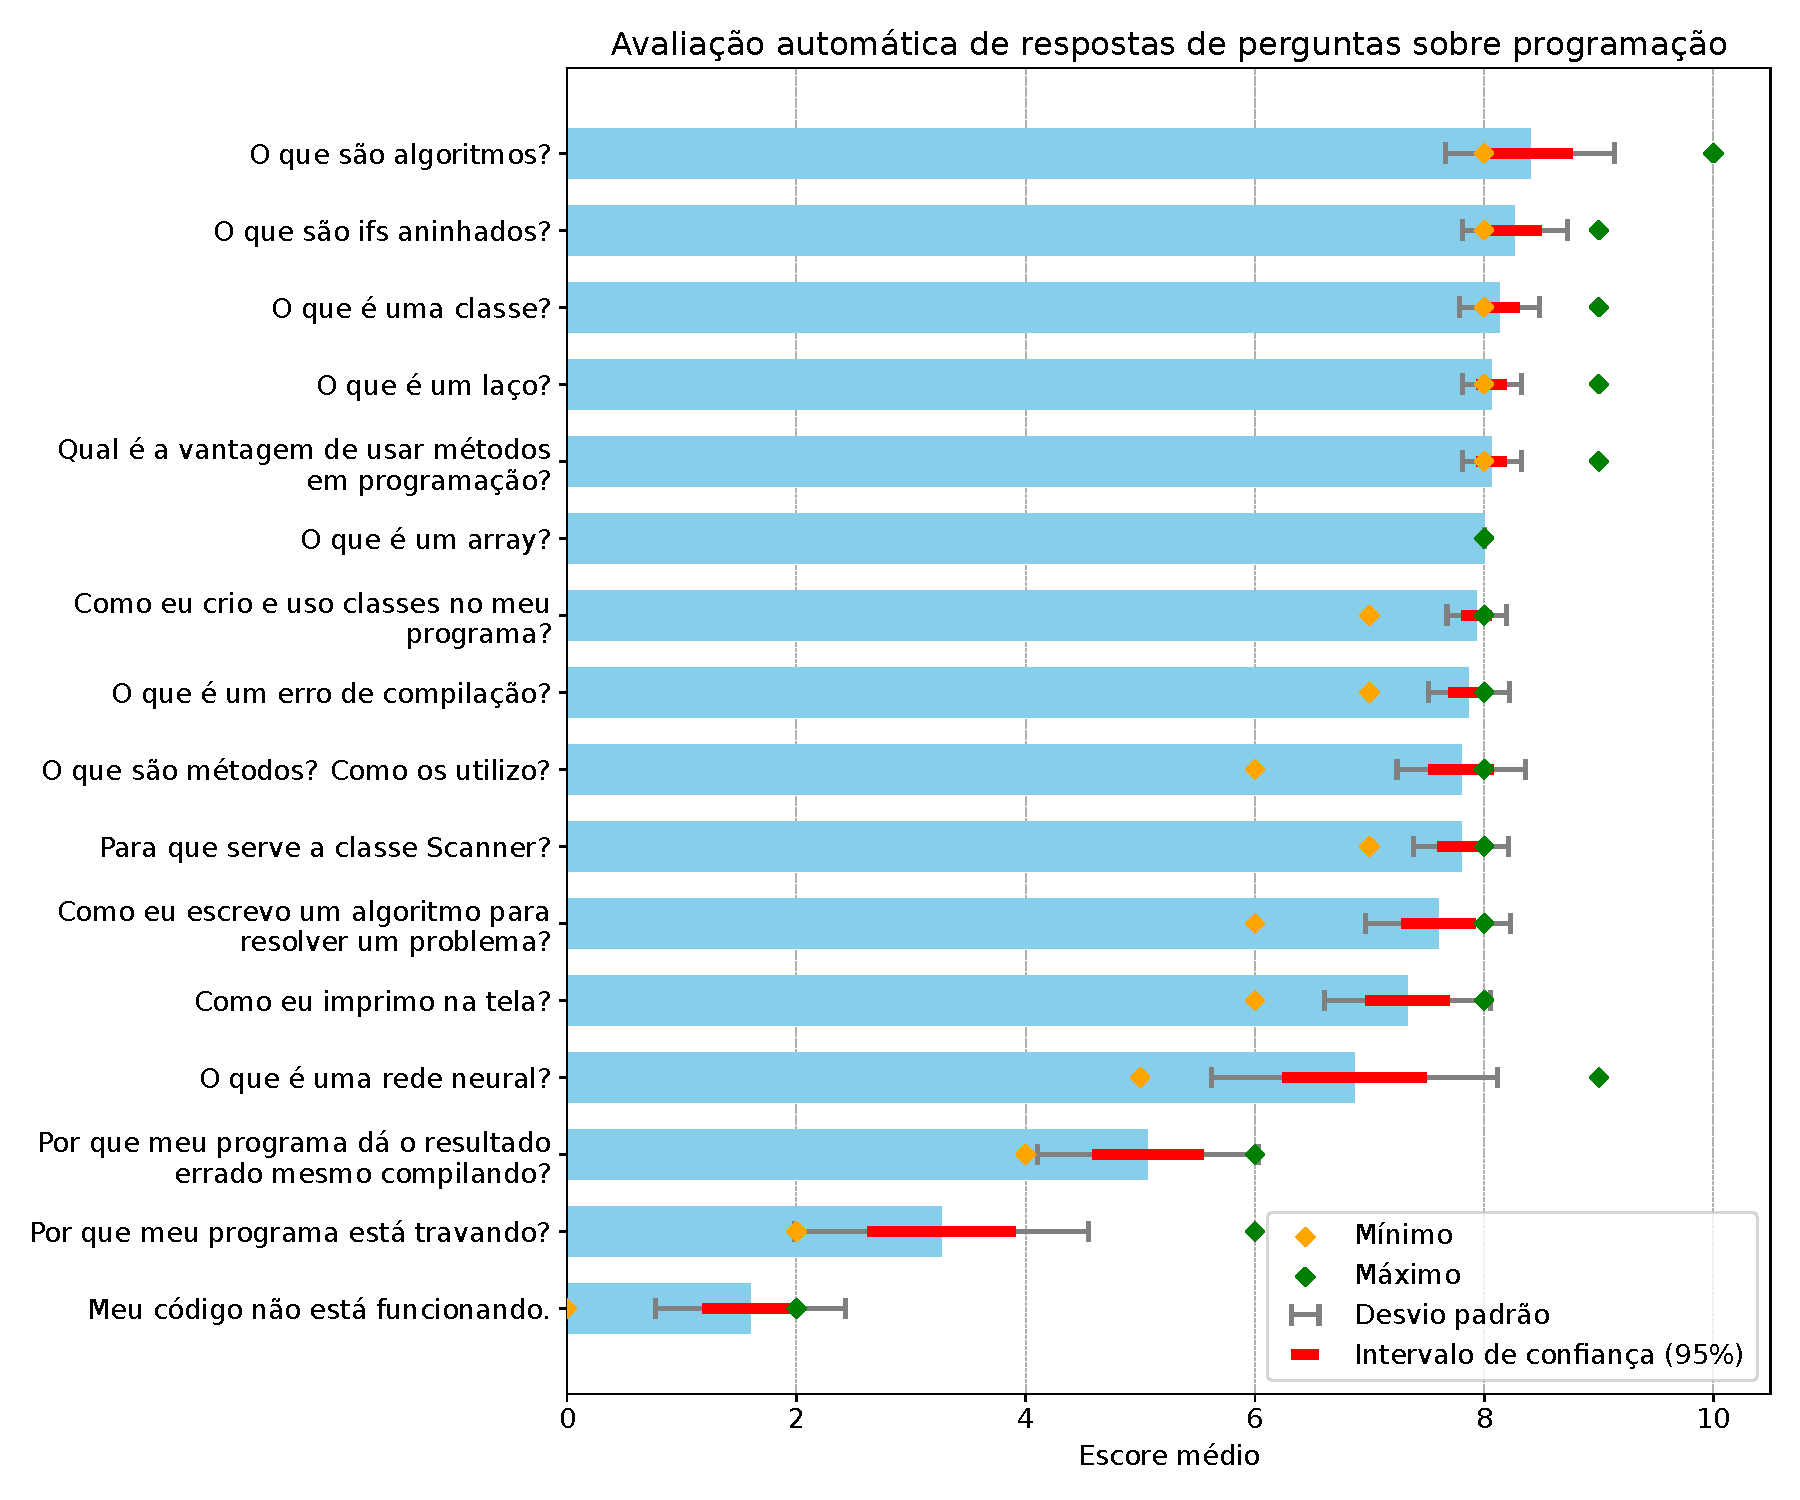
\includegraphics[width=\textwidth]{media/scores2.pdf}
    \caption{Excerto dos resultados obtidos por meio de avaliação automática das perguntas feitas ao sistema. Fonte: autor.\label{fig:resultados_perguntas_subset}}
\end{figure*}

A~\cref{fig:resultados_perguntas_subset} apresenta um excerto dos resultados obtidos por meio da avaliação automática.
O LLM avaliador --- LLaMA 3 70B Instruct ``puro'' --- foi instruído a dar uma nota de $0$ a $10$ para cada resposta, sendo $0$ a pior nota e $10$ a melhor.
É possível concluir que o modelo se saiu bem em responder perguntas utilizando o contexto, com notas acima de $7$ em quase todas as perguntas.
Também é possível notar que o avaliador deu notas mais baixas para perguntas onde o modelo solicitou mais informações ou não respondeu diretamente à pergunta, como ``Meu código não está funcionando'', onde o modelo muitas vezes respondeu com ``Desculpe'' e similares e pediu clarificações.
Ou seja, a avaliação automática é uma ferramenta útil, mas é necessário um olhar humano para avaliar as avaliações.

\subsubsection{Protocolo de teste manual}

\noindent%
O protocolo para testes conduzidos manualmente foi o seguinte: a partir da interface web, o modelo era questionado com uma das perguntas acima e a resposta era avaliada em relação à sua coesão, acurácia e relevância.
A coesão da resposta se refere à sua estrutura e organização, enquanto a acurácia se refere à correção dos fatos apresentados.
A relevância da resposta se refere à sua relação com a pergunta feita.

\subsection{Programação do sistema}

\noindent%
Toda a codificação do projeto está feita em Python\footnote{Disponível em:~\url{https://www.python.org}}, uma linguagem de programação de alto nível muito utilizada para projetos que envolvam inteligência artifical e aprendizado de máquina.
As bibliotecas relevantes utilizadas no projeto são o LlamaIndex e HuggingFace Transformers.
Bibliotecas como PyTorch, NumPy e afins são instaladas como dependências dessas bibliotecas principais.
Como se possui uma GPU da NVIDIA, a ``biblioteca'' CUDA foi instalada --- assim como o PyTorch com suporte a CUDA --- para que fosse possível utilizar a GPU nas tarefas de treinamento e inferência.
Localmente, o Mamba (similar ao Conda) foi utlizado para gestão das dependências.

A biblioteca LlamaIndex é utilizada para implementar o RAG\@.

\subsection{Técnicas de extensão de conhecimento}

\noindent%
Estender o conhecimento do modelo escolhido com os materiais didáticos disponíveis apresentou um desafio interessante: exstem diversas maneiras de se fazer isso, e cada uma delas tem suas vantagens e desvantagens, o que fez esse processo ser extremamente iterativo e experimental.
Inicialmente, foi feita uma análise dos materiais didáticos que seriam utilizados para extensão do conhecimento do modelo.
Concluída essa análise, foram levantadas as técnicas compatíveis com nosso \textit{dataset} e que trariam bons resultados sem a necessidade de muito poder computacional ou pré-tratamentos extensos (como rotulação manual, por exemplo).
Entre as técnicas no espaço de busca, foi escolhido o RAG como técnica de extensão do conhecimento do modelo.
Também foi considerado utilizar \textit{fine-tuning}, onde a documentação do LLaMA 3 indica \textit{parameter-efficient fine-tuning} (PEFT) com LoRA ou QLoRA antes de um processo que modifique todos os parâmetros para não ser necessário um poderil de recursos elevado.

Como mencionado anteriormente, o \textit{fine-tuning} envole o re-treinamento do modelo que está sendo refinado.
Além disso, sempre que forem adicionados novos conteúdos ao domínio --- por exemplo, um novo material de aula ---, é necessário o re-treinamento.
No entando, o \textit{fine-tuning} entrega um modelo pronto que não requer outras ferramentas para funcionar corretamente.
Mesmo assim, o RAG se mostra como a alternativa mais atraente por diversos motivos; entre eles:

\begin{enumerate}
    \item Nâo é necessário treinar um modelo massivo novamente, poupando recursos financeiros e computacionais.
    \item Permite a adaptação rápida a novos materiais didáticos.
    \item É de relativamente simples implementação e manutenção.
\end{enumerate}

Em outras palavras, o \textit{fine-tuning} congela o conhecimento de um modelo naquilo que está codificado na representação numérica de seus pesos.
Para adicionar conhecimento, é necessário ou treinar o modelo novamente ou utilizar RAG\@.
A desvantagem do RAG é que se faz necessária uma ferramenta auxiliar que faça essa extensão de conhecimento, adicionando um ponto a mais de falha na infraestrutura.

\subsubsection{Sobre \textit{fine-tuning}}

\noindent%
O \textit{fine-tuning} não foi escolhido mas também não foi descartado, pois ele é útil quando somente com RAG e \textit{prompt engineering} o modelo não performa como desejado, seja por questões comportamentais, de conhecimento, segurança, entre outros.
A Meta AI disponibiliza um \textit{script} oficial em seu repositório no GitHub para essa finalidade, assim como alguns \textit{datasets} de exemplo~\cite{llama3modelcard}.
Ao ler a documentação, se cita que ``[Utilizar] \textit{fine-tuning} com PEFT LoRA [\ldots] usando o \textit{dataset} OpenAssistant [e um tamanho de \textit{batch} de 4] [\ldots] demora em torno de dezesseis horas em uma única GPU e utiliza menos de \SI{10}{\giga\byte} de memória de GPU\@; mudar o tamanho de \textit{batch} para 8/16/32 utiliza 11/16/25 \SI{10}{\giga\byte} de memória de GPU''\@.
Com PEFT QLoRA demora em torno de seis horas e meia em uma única GPU e \SI{11}{\giga\byte} de memória de GPU\@.
A documentação cita também o projeto Axolotl~\cite{axolotl}, uma ferramenta que visa facilitar o processo de \textit{fine-tuning} que suporta diversos tipos de \textit{datasets} diferentes.
No término do processo de \textit{fine-tuning} ou de \textit{transfer learning} é retornado um modelo com sua arquitetura e pesos ajustados.
\ul{Esses pesos são o que fazem o modelo; sem eles, não há ``modelo''}.
São esses pesos que são distribuídos, assim como outras informações (exemplo: arquitetura), em plataformas como a HuggingFace.
Apesar de não ter sido escolhido nesse momento, aplicar \textit{fine-tuning} pode ser uma boa opção para melhorias desse projeto no futuro.

\subsection{Sobre RAG}

\noindent%
Para implementação do RAG foi utilizada a biblioteca LlamaIndex\footnote{Disponível em:~\url{https://www.llamaindex.ai}}, uma biblioteca de código aberto e de ampla utilização no mercado~\cite{Liu_LlamaIndex_2022}.
Existem outras bibliotecas de RAG como a LangChain\footnote{Disponível em:~\url{https://www.langchain.com}}~\cite{Chase_LangChain_2022}, mas o LlamaIndex foi escolhida por ter uma documentação aparentemente mais clara e coesa.
Tanto a LangChain quanto o LlamaIndex são bibliotecas conhecidas e utilizadas no mercado, então a escolha entre uma ou outra se deu por preferência pessoal.

Dentro da área de RAG existem diversas estratégias de busca e, similar ao restante do trabalho, escolher qual estratégia utilizar se deu por um processo iterativo.
Antes de determinar qual estratégia adotar, foi necessário escolher um modelo de \textit{embedding} que lidasse bem com dados textuais em português, inglês e código.

Brevemente e em altíssimo nível, um \textit{embedding} é uma representação de um texto (nesse contexto) em um vetor numérico.
Um modelo de \textit{embedding} é aquele que recebe texto como entrada e retorna um vetor de números que tentam capturar dados semânticos da entrada, permitindo assim uma busca semântica nos dados codificados.
Por exemplo, se um usuário fizer uma pergunta sobre laços, o vetor de \textit{embedding} resultante da pergunta será muito próximo do vetor de \textit{embedding} de textos que mencionam laços.

\subsection{Escolha do modelo de \textit{embedding}\label{sec:escolha_embedding}}

\noindent%
Foram considerados os modelos de \textit{embedding} mais conhecidos pela comunidade atualmente.
São eles:

\begin{itemize}
    \item \texttt{nomic-ai/nomic-embed-text-v1.5}~\cite{nussbaum2024nomic}
    \item \texttt{BAAI/bge-m3}~\cite{chen2024bge}
    \item \texttt{mixedbread-ai/mxbai-embed-large-v1}~\cite{emb2024mxbai}
    \item \texttt{intfloat/multilingual-e5-large}~\cite{wang2024multilingual}
    \item \texttt{intfloat/e5-mistral-7b-instruct}~\cite{wang2023improving}
\end{itemize}

Em seus testes,~\cite{borgne2024multilingualembed} compara esses e outros modelos.
Seus resultados demonstraram que o \texttt{BAAI/bge-m3} parece ser a melhor opção.
No entanto,~\cite{borgne2024multilingualembed} não testou \textit{corpus} em português, então podem haver divergências da realidade.
Foi escolhido o modelo \texttt{BAAI/bge-m3} para nosso caso de uso.

\subsection{Preparação dos dados\label{sec:prep_dados}}

\noindent%
Foram coletados os materiais didáticos da disciplina de Fundamentos da Programação, todos slides em formato PDF, para adicionar ao RAG\@.
Entretanto, alguns dos slides continham texto em formato de imagem, então foi necessário utilizar uma ferramenta de OCR nesses arquivos específicos.
No total, são menos de \SI{100}{\mega\byte} de dados crus.

O LlamaIndex disponibiliza diversas formas de carregar documentos para serem adicionados ao banco vetorial.
Entre elas, está sendo utilizada uma API da LlamaCloud\footnote{Disponível em:~\url{https://cloud.llamaindex.ai}} chamada LlamaParse, dos mesmos mantenedores do LlamaIndex.
Se optou pela LlamaParse pois ela possui um plano grátis, limitado a um número de páginas por dia com suporte a OCR e a diversas línguas, e também pode retornar os PDFs em formato Markdown.
Poderiam ter sido utilizadas ferramentas locais e de código aberto para atingir resultados semelhantes, mas optou-se por utilizar essa ferramenta, que apresentou excelentes resultados

O retorno em Markdown pode não parecer muito relevante a primeira vista, mas ele permite que seja feita uma revisão manual desses documentos antes de seguir para a próxima fase do processo, o armazenamento em um banco vetorial.
Essa revisão manual se fez necessária; os arquivos retornados foram verificados e modificados sempre que necessário (como erros de ortografia, formatação, ou até mesmo halucinações).
Por exemplo, a \cref{fig:llamaparse_lixo} foi um resultado obtido ao usar a LlamaParse em um dos PDFs, e a \cref{fig:llamaparse_corrigido} é o que se esperava desse mesmo arquivo.
Em contrapartida, a \cref{fig:llamaparse_tipos_de_erros} apresenta um exemplo de um resultado inalterado vindo diretamente dessa ferramenta.
O LlamaParse que adicionou o prefixo ``Erro de'' nos itens da lista nesse caso, pois fora instruído que eram slides de conteúdo de faculdade.
Isso pode indicar que o conteúdo dos arquivos está sendo analisado por um LLM e não uma ferramenta de OCR\@.

\begin{figure}[h]
    \centering
    \begin{minted}{markdown}
# Instruções de Saída

22
#

GMLmzd2

6C)- Criação das variáveis

OLw-#y

2 mc?

2Jx
    \end{minted}
    \caption{Resultado errôneo vindo do LlamaParse.\label{fig:llamaparse_lixo}}
\end{figure}

\begin{figure}[h]
    \centering
    \begin{minted}{markdown}
# Instruções de saída

Como o usuário deve informar a saída (tela)

System.out.print("Informe o nome:");
System.out.print(variavel);

# Criação das variáveis e constantes

Constantes são valores que não se alteram:

- Por convenção, seus identificadores são escritos em caixa alta.
- A declaração de constantes exige a palavra reservada final.

final tipo identificadorConstante = valor;
Exemplo: final double TAXA = 25;
    \end{minted}
    \caption{Resultado do LlamaParse esperado do mesmo arquivo utilizado na~\cref{fig:llamaparse_lixo}.\label{fig:llamaparse_corrigido}}
\end{figure}

\begin{figure}[h]
    \centering
    \begin{minted}{markdown}
Tipos de Erros

- Erro de Sintaxe: ocorre quando há um erro na estrutura do código, como falta de ponto e vírgula.
- Erro de Lógica: ocorre quando o código está correto, mas a lógica implementada não produz o resultado esperado.
- Erro de Tempo de Execução: ocorre durante a execução do programa, como divisão por zero.
- Erro de Semântica: ocorre quando o código está correto, mas não faz o que era esperado
    \end{minted}
    \caption{Resultado do LlamaParse sem alterações.\label{fig:llamaparse_tipos_de_erros}}
\end{figure}

Feita essa limpeza e revisão, se fez a inclusão desses documentos no banco de dados vetorial do LlamaIndex.
Mais uma vez, existem diversas formas de realizar essa importação.
Aqui são utilizadas diversas estratégias, ou transformações, de importação de dados: quebra do texto em \textit{chunks} (pedaços) menores, divisão hierárquica dos nodos, e afins.
A \cref{fig:llamaindex_md_read} apresenta um exemplo de importação desses arquivos em Markdown, assim como suas transformações.

\begin{figure}[h]
    \centering
    \begin{minted}{python}
from llama_index.core import (
  VectorStoreIndex,
  SimpleDirectoryReader
)
from llama_index.core.node_parser import (
  HierarchicalNodeParser,
  MarkdownNodeParser
)

reader = SimpleDirectoryReader('data/md/')
index = VectorStoreIndex.from_documents(
  reader.load_data(),
  transformations=[
    MarkdownNodeParser(),
    HierarchicalNodeParser.from_defaults(
      chunk_sizes=[2048, 512, 128],
      chunk_overlap=30
    ),
  ],
)
    \end{minted}
    \caption{%
    Leitura dos arquivos em Markdown para serem adicionados ao banco vetorial (\texttt{index}) com transformações de quebra hierárquica.\label{fig:llamaindex_md_read}}
\end{figure}

Analisando a \cref{fig:llamaindex_md_read}, se vê que está sendo criado um \texttt{VectorStoreIndex} da biblioteca LlamaIndex chamado \texttt{index}, e é a partir dele que será criado o motor de \textit{chat} ou conversação utilizado pela Pipeline nas próximas seções.

\subsection{LlamaIndex e adicionais\label{sec:indo_alem_do_llamaindex}}

\noindent%
A implementação utilizando somente LlamaIndex, por si só, já possui funcionalidades suficientes para atender o requisito básico deste estudo, que é utilizar inteligência artificial como apoio ao aprendizado de programação.
Para tal, basta fazer uso da \texttt{VectorStoreIndex} apresentada na~\cref{fig:llamaindex_md_read} e convertê-la para um motor de conversação com a função \mintinline{python}|VectorStoreIndex.as_chat_engine|.
A \cref{fig:llamaindex_engine_react} apresenta um exemplo de uso, onde a resposta obtida foi:

\begin{quote}{LLaMA 3, ReAct}
Um algoritmo é um conjunto finito de regras, bem definidas, para a solução de um problema em um tempo finito.
Ou, de outra forma, é um texto que contém uma série de ações primitivas que, quando executadas, operam sobre os dados, transformando-os em saídas.
\end{quote}

O modelo gerador da resposta anterior foi o LLaMA 3 70B Instruct sem quaisquer modificações de hiperparâmetros ou \textit{prompt engineering}, munido com o contexto dos conteúdos de aula mencionados na~\cref{sec:prep_dados}.

Importante mencionar a opção \texttt{chat\_mode} do motor de conversação.
A documentação do LlamaIndex entra em detalhes sobre cada opção.
A opção \mintinline{python}|ChatMode.REACT| usa o motor de busca como ferramenta de apoio ao LLM, decidindo se vai ou não fazer uma busca contextual.
Essa opção permite que o modelo responda a perguntas que não estão explicitamente definidas em seus provedores de contexto.
A opção \mintinline{python}|ChatMode.CONDENSE_PLUS_CONTEXT| condensa o histórico da conversa com o usuário em uma única pergunta, busca em seus provedores de contexto informações adicionais sobre aquele assunto e então repassa ao LLM o contexto encontrado e a mensagem \textit{verbatim} do usuário.
Ambas opções foram testadas e ambas trouxeram bons resultados.
A~\cref{fig:llamaindex_engine_condense_plus_context} apresenta um exemplo de uso da opção \mintinline{python}|ChatMode.CONDENSE_PLUS_CONTEXT|, onde a resposta obtida foi:

\begin{quote}{LLaMA 3, Condense Plus Context}
Um algoritmo é um conjunto finito de regras bem definidas para a solução de um problema em um tempo finito.
Além disso, também é definido como um texto (como uma receita de bolo) onde cada linha contém uma ação primitiva (ação elementar passível de execução por um humano ou uma máquina).
\end{quote}

O modo Condense Plus Context, por avaliação experiencial, apresentou resultados um pouco mais satisfatórias do que o modo ReAct, consistentemente demonstrando um entendimento do contexto oferecido pelo RAG e usuário.
Um exemplo disso está nas respostas anteriores, onde o Condense Plus Context menciona ``receita de bolo'', um exemplo que foi dado em um dos slides de aula.
Em outras palavras, esse modo repassou de maneira mais explícita as informações providas pelo RAG\@.
Sendo assim, a opção \mintinline{python}|ChatMode.CONDENSE_PLUS_CONTEXT| foi escolhida para a implementação final.

Um ponto de atenção ao utilizar LLMs em línguas diferentes daquelas em que foram treinados é a perda de contexto e detalhes específicos da língua, pois internamente é utilizado um modelo de tradução automática para converter o texto em português para o inglês.
Essa tradução não é perfeita, podendo levar a respostas imprecisas.

\begin{figure}[h]
    \centering
    \begin{minted}{python}
engine = index.as_chat_engine(
    chat_mode=ChatMode.REACT,
    verbose=True)

response = engine.chat('O que é um algoritmo?')
print(response)
    \end{minted}
    \caption{Utilizando o LlamaIndex como motor de conversação no modo \mintinline{python}|ChatMode.REACT|.
    A saída está apresentada na \autoref{sec:indo_alem_do_llamaindex}, modo ReAct.\label{fig:llamaindex_engine_react}}
\end{figure}

\begin{figure}[h]
    \centering
    \begin{minted}{python}
from llama_index.core.chat_engine import (
    CondensePlusContextChatEngine
)

cls = CondensePlusContextChatEngine
engine = cls.from_defaults(
    index.as_retriever(),
    verbose=True
)

response = engine.chat('O que é um algoritmo?')
print(response)
    \end{minted}
    \caption{Utilizando o LlamaIndex como motor de conversação no modo \mintinline{python}|ChatMode.CONDENSE_PLUS_CONTEXT|.
    A saída está apresentada na \autoref{sec:indo_alem_do_llamaindex}, modo Condense Plus Context.
    Só se define \texttt{cls} na linha 5 para evitar extensão horizontal.\label{fig:llamaindex_engine_condense_plus_context}}
\end{figure}

Para demonstrar que o sistema consegue manter um histórico e um contexto de conversa, foi perguntado novamente o que é um algoritmo, e a resposta obtida foi:

\begin{quote}{LLaMA 3, Condense Plus Context}
Você já fez essa pergunta anteriormente!

Lembre-se de que um algoritmo é um conjunto finito de regras, bem definidas, para a solução de um problema em um tempo finito.
Ou, de uma forma mais coloquial, é como uma ``receita de bolo'' onde cada linha contém uma ação primitiva.

Mas, como você já conhece essa definição, vamos ir um pouco mais além! Você sabe que os algoritmos podem ser classificados em diferentes tipos, como algoritmos de ordenação, algoritmos de busca, algoritmos de criptografia, entre outros?

Você gostaria de explorar mais sobre os diferentes tipos de algoritmos e suas aplicações? Ou talvez você queira saber como os algoritmos são projetados e implementados em diferentes linguagens de programação?
\end{quote}

Essa resposta demonstra que o sistema, além de ser capaz de manter um histórico, tenta instigar e guiar o usuário para um aprendizado mais profundo.
O modelo foi instruído a apresentar esse comportamento de ``guia'' por sua \textit{prompt} de sistema (\cref{fig:system_prompt}).

A abordagem apresentada nas~\cref{fig:llamaindex_engine_react,fig:llamaindex_engine_condense_plus_context} é limitada à linha de comando (CLI), Jupyter Notebooks e afins.
Em outras palavras, não é necessariamente amigável para todos os usuários.
Ela também não apresenta mecanismos de controle de acesso, interface web, monitoramento de uso, e outras funcionalidades desejadas neste projeto.
Para atingir esses requisitos se faz necessária uma interface de usuário.
Neste trabalho é utilizada a OpenWebUI\footnote{Disponível em:~\url{https://openwebui.com}}, uma interface web de código aberto desenvolvida pela comunidade e de simples instalação e configuração~\cite{openwebui}.
Outras interfaces populares são a AnythingLLM\footnote{Disponível em:~\url{https://useanything.com}} e o LLM Studio\footnote{Disponível em:~\url{https://lmstudio.ai}}.

\subsection{Interface web}

\noindent%
A OpenWebUI, interface web em utilização, é um projeto maduro que possui muitas opções atraentes para este estudo.
Além disso, ela possui um sistema de RAG próprio que poderia ter sido utilizado mas não apresentou resultados satisfatórios durante o período de testes.
Para o RAG, foi implementada uma \textit{pipeline} com base no \textit{framework} Pipelines apresentado nas seções a seguir.
Atrativos da OpenWebUI incluem:

\begin{itemize}
    \item Integração direta com Ollama.
    \item Controle de acesso de usuários.
    \item Limitações de quantidade de requisições.
    \item Integração com sistemas de autenticação (SSO) como Azure Entra ID e OAuth.
    \item Modificação de modelos do Ollama diretamente pela interface.
    \item Execução em Docker.
\end{itemize}

A~\cref{fig:openwebui_example} apresenta a página inicial de um usuário autenticado na OpenWebUI\@.
Já a~\cref{fig:openwebui_example_2} apresenta um exemplo de uso, onde o usuário pergunta ``O que é um algoritmo?\,'' e o sistema o responde.
Essa interface é, na percepção do autor, extremamente intuitiva e remete à interface do ChatGPT da OpenAI\@.

\begin{figure*}[ht!]
    \centering
    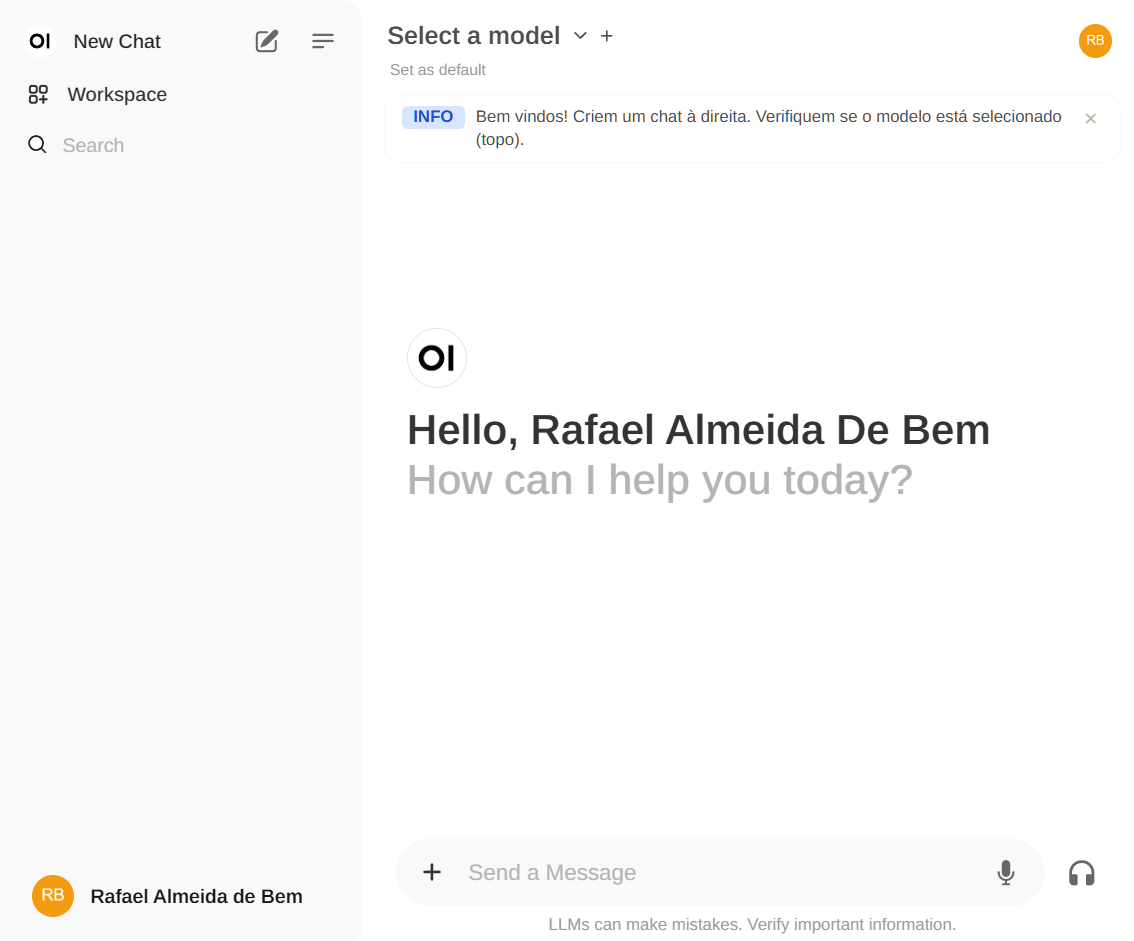
\includegraphics[width=\textwidth]{media/openwebui_example.png}
    \caption{Página inicial da OpenWebUI\@. Fonte: autor.\label{fig:openwebui_example}}
\end{figure*}

\begin{figure*}[h]
    \centering
    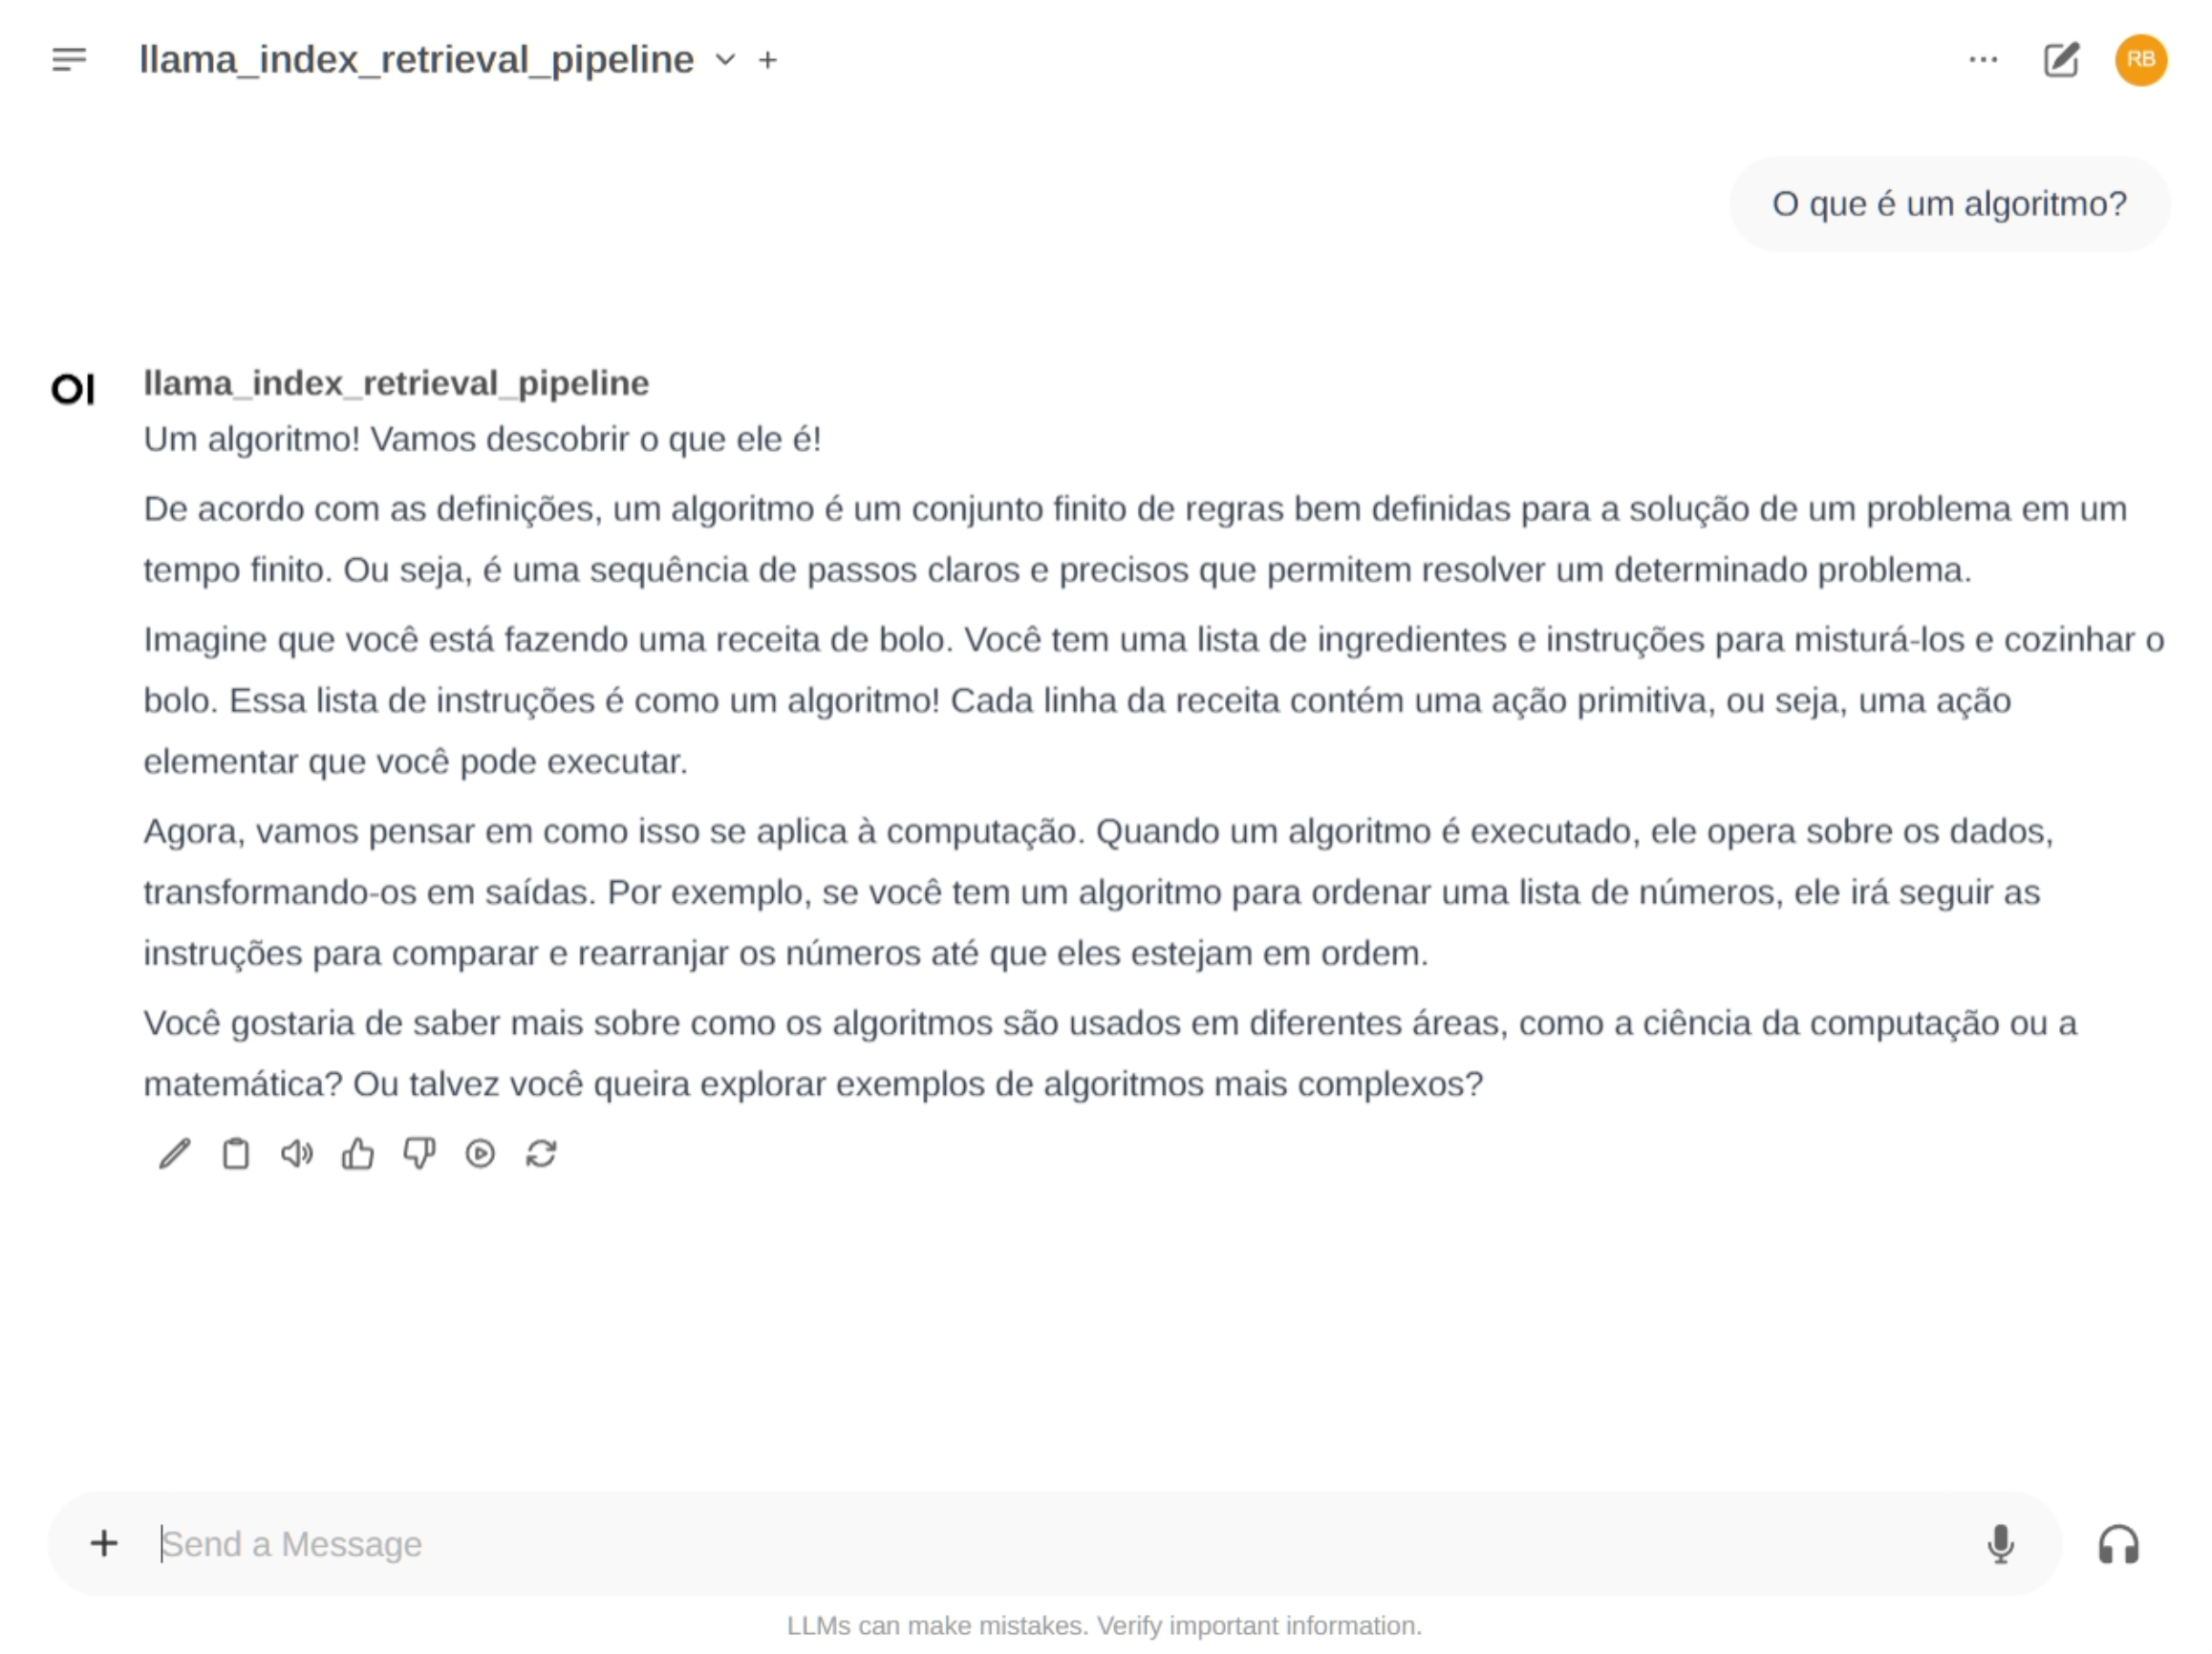
\includegraphics[width=\textwidth]{media/openwebui_example_2.png}
    \caption{Exemplo de uso da OpenWebUI\@. Fonte: autor.\label{fig:openwebui_example_2}}
\end{figure*}

\subsection{O que são \textit{pipelines}?\label{sec:o_que_sao_pipelines}}

\noindent%
Em poucas palavras, \textit{pipelines} são uma sequência de ações a serem tomadas a fim de gerar um resultado a partir de uma entrada.
Esse conceito é utilizado em muitas áreas da computação.
Alguns exemplos são as \textit{pipelines} de entrega contínua (GitHub CI/CD, GitLab pipelines, Bamboo), \textit{pipelines} de processamento de dados, \textit{pipelines} de transformações de dados do LlamaIndex, entre outras.
Todos esses exemplos recebem uma entrada, atuam sobre ela e geram um resultado.
Por exemplo, as \textit{pipelines} de entrega contínua (CI/CD) recebem de entrada um código fonte, o compilam, executam testes unitários e afins, assinam o binário e ``entregam'' um ou vários executáveis para serem distribuídos.

\subsection{LlamaIndex e a OpenWebUI}

\noindent%
Para que fosse possível integrar nosso sistema RAG com a interface web escolhida, foi necessário fazer uso de uma \textit{pipeline} personalizada.
Os mantenedores do projeto da OpenWebUI desenvolveram um \textit{framework} agnóstico à interface chamado Pipelines\footnote{Disponível em:~\url{https://docs.openwebui.com/pipelines}} que permite a criação de fluxos de trabalho personalizados para quaisquer interfaces e modelos.
Por exemplo, é possível criar uma \textit{pipeline} que executa antes do modelo ser chamado e filtre perguntas indevidas, ou uma que executa após o modelo ser chamado e filtre respostas de baixa coesão.
Também é possível criar \textit{pipelines} que adicionam contexto às perguntas, e é nessa área que o RAG desenvolvido se encaixa.
A \cref{fig:rag_pipeline} demonstra dois casos de uso de \textit{pipelines}: um filtro (superior) e um ``qualquer'' (inferior), que executa qualquer código antes ou depois da inferência do modelo, demonstrando as capacidades de extensão desse sistema.

Nota sobre a terminologia: ``\textit{pipeline}'', em itálico, é o conjunto de ações a serem tomadas (\autoref{sec:o_que_sao_pipelines}), e ``Pipelines'', com capitalização, é o \textit{framework} desenvolvido pela OpenWebUI\@.

\begin{figure*}[h]
    \centering
    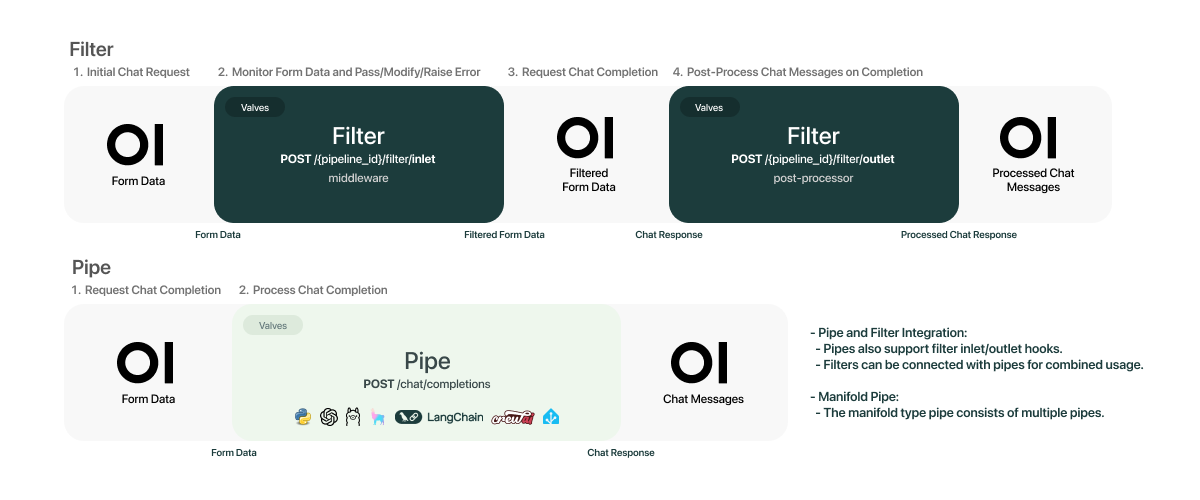
\includegraphics[width=\textwidth,clip,trim=40 40 40 40]{media/openwebui_pipelines_workflow.png}
    \caption{Exemplos de \textit{pipelines}. Fonte:~\cite{openwebui}\label{fig:rag_pipeline}}
\end{figure*}

A OpenWebUI se conecta à uma instância do Pipelines como se fosse uma API de inferência qualquer.
Além disso, dependendo do tipo de \textit{pipeline}, cada \textit{pipeline} de uma determinada instância do Pipelines aparece na OpenWebUI como se fosse um LLM auto-contido.
No âmbito desse estudo, a \textit{pipeline} desenvolvida aparece na lista de modelos como se fosse um modelo qualquer (\autoref{fig:openwebui_pipeline_model_list}).

\begin{figure}[h]
    \centering
    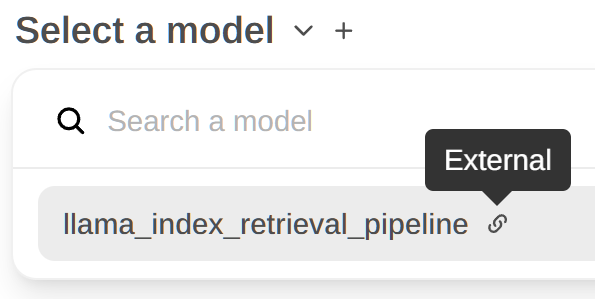
\includegraphics[width=\columnwidth]{media/openwebui_pipeline_model_list.png}
    \caption{Exemplo da \textit{pipeline} na lista de modelos da OpenWebUI\@. Fonte: autor.\label{fig:openwebui_pipeline_model_list}}
\end{figure}

Fazendo uso do Pipelines, a OpenWebUI não se conecta à instância do Ollama e sim à instância do Pipelines.
Isso traz, infelizmente, a desvantagem de que se perde o paralelismo de inferência implementado pela OpenWebUI ao se conectar a diversas instâncias do Ollama.
No entando, esse paralelismo pode ser re-implementado pela própria \textit{pipeline} desenvolvida, mas está fora do escopo deste trabalho.

\subsection{Integração do LlamaIndex à \textit{pipeline}}

\noindent%
Para integrar o LlamaIndex à \textit{pipeline} do OpenWebUI, foi criada uma \textit{pipeline} que executa as buscas em um banco vetorial antes da inferência do modelo.
A \textit{pipeline} foi desenvolvida utilizando uma classe do próprio \textit{framework} Pipelines e adicionada a OpenWebUI através de integrações existentes.
O código desenvolvido pode ser encontrado na íntegra no repositório deste projeto\footnote{Disponível em:~\url{https://tcc.debem.dev}}.

Foram adicionadas diversas opções na \textit{pipeline} desenvolvida, ou ``válvulas'' na terminologia do Pipelines, para que se pudesse modificar o funcionamento do sistema sem precisar reiniciar os serviços.
Algumas opções são visíveis na \autoref{fig:openwebui_pipeline_config}.

Uma importante configuração e, de certa forma, decisão arquitetônica, é como e onde rodar o modelo.
A \textit{pipeline} espera um endereço, uma URL, para conectar-se ao Ollama.
Esse endereço pode ser local (\texttt{localhost}, \texttt{host.docker.internal}) ou remoto, e depende da infraestrutura existente ou planejada.
Também adicionou-se suporte a não utilizar o Ollama e sim outros sistemas de execução de modelos como HuggingFace Transformers, vLLM, e até mesmo serviços como Groq e OpenAI\@.

A parte do código da \textit{pipeline} desenvolvida que faz o RAG é praticamente uma cópia dos códigos do LlamaIndex apresentados nas seções anteriores.
Uma mudança significativa é a persistência do banco vetorial em um contexto de armazenamento (\texttt{StorageContext}) para que não seja necessário gerar os \textit{embeddings} dos arquivos toda vez que o sistema reiniciar.
Ao invés disso, eles são persistidos através desse \texttt{StorageContext}, classe que permite o salvamento e carregamento dos dados em qualquer sistema compatível com a especificação fsspec --- uma biblioteca que especifica uma interface unificada para interação com tipos de sistemas de arquivos diferentes (memória, disco, Amazon S3, FTP, \ldots) através de uma API comum~\cite{Liu_LlamaIndex_2022,fsspec}.
Por mais que a implementação atual utilize armazenamento em disco, a opção de armazenamento em nuvem é fortemente sugerida para ambientes de produção.

\subsection{Modificação da \textit{prompt} de sistema do modelo}

\noindent%
Não basta apenas munir o modelo com informações e esperar que ele responda da maneira desejada sem instruí-lo devidamente.
Para que o modelo responda de maneira coerente e contextualizada, é necessário fornecer instruções claras e específicas sobre o que se espera dele.
Isso pode ser obtido por diversas maneiras, e uma delas é a modificação da \textit{prompt} de sistema do modelo.
A \textit{prompt} de sistema, também conhecida como ``papel do sistema'', é uma sequência de texto que é fornecida ao modelo juntamente com a pergunta do usuário, e é utilizada para instruir o modelo sobre o que se espera dele.
Cada LLM se comporta de uma maneira diferente; sendo assim, é necessário refinar e testar diversos tipos de \textit{prompts} de sistema no modelo selecionado para determinar qual é o mais eficaz para a tarefa desejada~\cite{bozkurt2024tell,brown2020language,radford2019language,bsharat2023principled}.
A área de \textit{prompt engineering}, ou engenharia de \textit{prompts}, é a área da IA focada especificamente em criar \textit{prompts} eficazes para modelos de linguagem, e é essencial para o futuro dos LLMs.
Segundo~\cite{radford2019language}, \textit{prompt engineering} é a arte de se comunicar e interagir com IA Generativa\footnote{\textit{Prompt engineering is the art of communicating and interacting with generative AI}}.

Para se obter uma \textit{prompt} de sistema eficiente, foram aplicadas diversas técnicas diferentes baseadas em~\cite{doi:10.1080/10875301.2023.2227621,lo2023clear} e~\cite{openaipromptengineering,beurer2023prompting,mao2023large} como \textit{zero-shot}, persona ou \textit{role-play} e \textit{chain-of-thought}.
Em~\cite{doi:10.1080/10875301.2023.2227621,lo2023clear} é apresentado o acrônimo CLEAR, que define um \textit{framework} de como uma \textit{prompt} deve ser: concisa, lógica, explícita, adaptativa e reflectiva.
Já~\cite{openaipromptengineering} apresenta um guia com táticas e estratégias para se criar \textit{prompts} eficazes para modelos de linguagem, e se alinha com o \textit{framework} CLEAR\@.
A \autoref{tab:openaiprompts} apresenta alguns exemplos de \textit{prompts} ruins e suas versões melhoradas~\cite{openaipromptengineering}.

\begin{table}
    \caption{Exemplos de \textit{prompts} ruins e suas versões melhoradas. Fonte:~\cite{openaipromptengineering}.\label{tab:openaiprompts}}
    \centering
    \begin{tabularx}{\columnwidth}{XX}
        \toprule
        \textbf{Pior} & \textbf{Melhor} \\
        \midrule
        How do I add numbers in Excel?                  & How do I add up a row of dollar amounts in Excel? I want to do this
                                                          automatically for a whole sheet of rows with all the totals ending
                                                          up on the right in a column called ``Total''.\\
        \midrule
        Who's president?                                & Who was the president of Mexico in 2021, and how frequently are
                                                          elections held?\\
        \midrule
        Write code to calculate the Fibonacci sequence. & Write a TypeScript function to efficiently calculate the Fibonacci
                                                          sequence. Comment the code liberally to explain what each piece does
                                                          and why it's written that way.\\
        \bottomrule
    \end{tabularx}
\end{table}

Outra estratégia utilizada foi a de fazer o modelo adotar uma personalidade, ou ``persona'', que é uma maneira de fazer o modelo atuar em um determinado papel (\textit{role-play})~\cite{kong2023better}.
Essa técnica foi muito eficaz.
Por exemplo, se pode dizer ao modelo, ``Atue como um comediante'' ou ``Você é um tutor de matemática excelente''~\cite{openaipromptengineering}.

Como mencionado anteriormente, cada LLM se comporta de uma maneira diferente e é necessário testar cada caso de maneira iterativa para determinar qual é a melhor \textit{prompt} de sistema para a tarefa desejada.
Ou seja, o LLaMA 3 se comporta de uma maneira única.
Na documentação do LLaMA 3 existe uma seção específica sobre as técnicas de \textit{prompt engineering} que são mais eficazes para esse modelo.
Segundo~\cite{kong2023better}, LLMs se comportam bem quando são dados um papel específico a cumprir, e a documentação do LLaMA 3 sugere a mesma abordagem~\cite{llama3modelcard}.
Outras técnicas como \textit{chain-of-thought}~\cite{wei2022chain} e limitação de \textit{tokens} extrâneos também são sugeridas e foram aplicadas durante o desenvolvimento do sistema.

\begin{figure*}[ht]
    \centering
    \begin{minted}{markdown}
Act as a teacher assistant and answer questions using the provided context.
Your goal is to help students and teachers by providing cohesive and correct responses based on educational material, while applying guided learning techniques.
Give examples and cite the context whenever possible.
Don't mention 'according to the context' or anything related to that, ever.
## Instructions
1. External Information: Use external information from the vector database to answer questions. Select the most relevant and reliable information available.
2. Guided Learning Techniques: Avoid giving direct answers. Instead, guide the user through the learning process, encouraging critical thinking and discovery.
3. Coherent and Correct Responses: Ensure that all responses are coherent and correct, strictly following the educational material provided.
4. Inference Capability: Use your skills to accurately deduce and infer information.
5. User-Friendly Interface: Be easy to use and access. Provide clear and well-structured responses suitable for a web interface.
6. Value Addition: Add value for both students and teachers. Offer useful insights, pedagogical guidance, and support the teaching-learning process.
7. Best-effort: The user is a beginner, and may use terms incorrectly or in other languages. Do your best to understand what they mean.
## User Interaction
- Interactive Guidance: Ask the user if they would like more details or additional examples.
- Encourage Exploration: Motivate users to explore more about the topic by suggesting additional resources or related questions.
## Additional Information
- Utilize the context provided in the vector database to enrich your responses.
- Ensure your answers are always up-to-date and based on the most recent information available.
Your mission is to provide a rich and interactive learning experience, helping students and teachers achieve their educational goals efficiently and effectively.
    \end{minted}
    \caption{\textit{Prompt} do sistema utilizada para gerar os resultados apresentados. Fonte: autor.\label{fig:system_prompt}}
\end{figure*}

A \textit{prompt} de sistema ``final'' utilizada neste trabalho é apresentada na~\cref{fig:system_prompt}.
Para montar essa \textit{prompt}, aplicou-se todas as técnicas de \textit{prompt engineering} previamente mencionadas, assim como uma abordagem iterativa.
Seguindo a documentação do LLaMA 3, a \textit{prompt} foi dividida em seções, cada uma com um propósito específico.
Não foram adicionados exemplos de respostas esperadas (\textit{few-shot prompting}) pois não foram necessários para a tarefa em questão.
Para evitar que o modelo diga ``segundo o contexto'', ``de acordo com o contexto'', ou algo similar, foi adicionado um item específico na \textit{prompt} que proíbe o modelo de fazer isso.
Ao fim das intruções e regras, foi adicionado um resumo do que se espera do modelo, e o papel que ele deve desempenhar, para reforçar o que se espera dele~\cite{kong2023better,wei2022chain,beurer2023prompting,mao2023large}.

Apesar de \textit{prompt engineering} ser uma técnica poderosa, ela não é uma solução mágica e possui limitações.
Nesses casos, pode ser necessário tomar uma abordagem diferente, como as modificações de hiperparâmetros do modelo, ou até mesmo a troca do modelo por um mais adequado.

\subsection{Hiperparâmetros do LLM e outras opções}

\noindent%
Caso o sistema não apresente resultados satisfatórios, é possível modificar tanto os parâmetros do RAG quanto os hiperparâmetros do modelo.
No caso do LLaMA 3, os hiperparâmetros \texttt{temperature} e \texttt{top\_p} são modificáveis.
Resumidamente, o \texttt{top\_p} controla o espaço de busca do vocabulário durante a geração, e a \texttt{temperature} controla a aleatoriedade desse vocabulário.
Uma \texttt{temperature} de 0 produz resultados \textit{quase} determinísticos~\cite{llama3modelcard}.

\subsection{Fluxo básico de dados}

\noindent%
A~\cref{fig:flow_chat} apresenta um diagrama do fluxo de chamadas no sistema desenvolvido quando o usuário envia uma mensagem.
Assume-se que a \textit{pipeline} e o RAG já haviam sido iniciados; ou seja, não é a primeira inicialização, pois nesses casos é necessário gerar o banco vetorial.
Um ``nodo'' refere-se a um pedaço (\textit{chunk}) de um documento já indexado.
As respostas geradas pelo modelo são um conjunto cumulativo de \textit{tokens}, onde cada iteração adiciona alguns \textit{tokens} a esse conjunto.
A cada iteração, esses \textit{output tokens} (\textit{tokens} de saída) são enviados à \textit{pipeline}, e por isso essas chamadas estão dentro de um \textit{loop}.
O usuário interage com a interface web, que envia a mensagem para a \textit{pipeline} do Pipelines.
A \textit{pipeline} executa a busca no banco vetorial do RAG, e então envia a pergunta e o contexto para o modelo.
O modelo gera uma resposta, que é enviada de volta para a \textit{pipeline}, que então a envia de volta para a interface web.

\begin{figure*}[ht]
    \centering
    \begin{sequencediagram}
        \newthread{web}{Interface Web}
        \newinst[2.5]{pipe}{Pipeline}
        \newinst[2.5]{rag}{RAG}
        \newinst[2.5]{model}{Modelo}

        \begin{messcall}{web}{Histórico}{pipe}
        \end{messcall}

        \begin{call}{web}{Pergunta}{pipe}{Resposta}
            \begin{call}{pipe}{Pergunta}{rag}{Embeddings}
            \end{call}\postlevel%

            \begin{call}{pipe}{\shortstack{Busca no\\banco vetorial}}{rag}{Contexto}
                \begin{callself}{rag}{Embeddings}{Nodos relevantes}\end{callself}
                \begin{callself}{rag}{Nodos relevantes}{Contexto}\end{callself}
            \end{call}\postlevel%

            \begin{call}{pipe}{Pergunta e contexto}{rag}{Nova prompt}
            \end{call}\postlevel%

            \begin{call}{pipe}{System prompt, nova prompt, histórico}{model}{Fim da inferência}
                \begin{sdblock}{Stream/loop}{Consumo dos tokens de entrada}
                    \begin{callself}{model}{Input tokens}{Output}
                    \end{callself}
                    \mess{model}{Resposta gerada}{pipe}
                \end{sdblock}
            \end{call}
        \end{call}
    \end{sequencediagram}
    \caption{%
    Diagrama UML do fluxo de dados no sistema desenvolvido. Fonte: autor.\label{fig:flow_chat}}
\end{figure*}

\subsection{Integração com sistemas de \textit{learning analytics}\label{sec:learning_analytics}}

\noindent%
O sistema desenvolvido integra-se com sistemas de \textit{learning analytics} para monitorar mensagens de usuários e gerar relatórios de desempenho.
A integração demonstrada a seguir utiliza a \textit{pipeline} para enviar mensagens para uma API externa básica.
Essa API foi escrita em Python e utiliza a biblioteca FastAPI\footnote{%
Disponível em:~\url{https://fastapi.tiangolo.com}} para criar um servidor web que recebe mensagens e as armazena em um banco de dados PostgreSQL\footnote{%
Disponível em:~\url{https://www.postgresql.org}}.
As mensagens armazenadas seguem o formato apresentado na~\cref{fig:api_messages}, uma rota que adiciona um par  mensagem e resposta a determinado usuário.
Essa API é um exemplo básico e não deve ser utilizada em ambientes de produção sem modificações significativas.

Para agregar valor, implementou-se também uma rota que retorna todos os tópicos das conversas armazenadas para um determinado usuário.
Essa rota foi criada como uma prova de conceito para demonstrar a integração com sistemas de \textit{learning analytics}.
A~\cref{fig:api_topics} apresenta o formato dessa rota.
Ao acessar essa rota com o \texttt{student\_id} do usuário que enviou as mensagens ``O que é um algoritmo?\,'' e ``Como eu faço um \texttt{if} em Java?\,'', esse serviço retornou os seguintes tópicos:

\begin{itemize}
    \item Algoritmos
    \item Programação
    \item Linguagem Algorítmica
    \item Estrutura de Controle de Fluxo
\end{itemize}

A conversa repassada ao gerador de tópicos envolveu os tópicos retornados, logo a resposta foi satisfatória.

\begin{figure}[ht]
    \centering
    \begin{apiRoute}{post}{/api/\{student\_id\}/messages/}{Adiciona uma mensagem ao usuário.}
        \begin{routeParameter}
            \routeParamItem{student\_id}{UUID}{Identificador do usuário na OpenWebUI.}
        \end{routeParameter}

        \begin{routeRequest}{application/json}
            \begin{routeRequestBody}
{
    "content": "string",
    "response": "string"
}
            \end{routeRequestBody}
        \end{routeRequest}

        \begin{routeResponse}{application/json}
            \begin{routeResponseItem}{200}{OK}
                \begin{routeResponseItemBody}
{
  "content": "string",
  "response": "string",
  "id": 0,
  "student_id": UUID
}
                \end{routeResponseItemBody}
            \end{routeResponseItem}
        \end{routeResponse}
    \end{apiRoute}
    \caption{%
    Formato das mensagens enviadas pela \textit{pipeline} para a API de \textit{learning analytics}. Fonte: autor.\label{fig:api_messages}}
\end{figure}

\begin{figure}[ht]
    \centering
    \begin{apiRoute}{get}{/api/\{student\_id\}/generate\_topics}{Gera tópicos das conversas de um usuário.}
        \begin{routeParameter}
            \routeParamItem{student\_id}{UUID}{Identificador do usuário na OpenWebUI.}
        \end{routeParameter}

        \begin{routeResponse}{application/json}
            \begin{routeResponseItem}{200}{OK}
                \begin{routeResponseItemBody}
[ "string" ]
                \end{routeResponseItemBody}
            \end{routeResponseItem}
        \end{routeResponse}
    \end{apiRoute}
    \caption{%
    Rota de geração automática de tópicos da conversa entre um usuário e o sistema. Fonte: autor.\label{fig:api_topics}}
\end{figure}

Essas funcionalidades já satisfazem a prova de conceito de integração com sistemas de \textit{learning analytics} desejada.
O código completo da API, assim como sua configuração de Docker Compose, encontra-se no repositório deste projeto\footnote{Disponível em:~\url{https://tcc.debem.dev}}.
As modificações necessárias na \textit{pipeline} para integrar com essa API também estão disponíveis no repositório, na função \mintinline{python}|Pipeline.outlet()|.

\section{Implantação em ambientes de teste\label{sec:deploy_test}}

\noindent%
Nessa seção é apresentado um exemplo de implantação (\textit{deployment}) do sistema completo em um ambiente de testes.
Durante o desenvolvimento do trabalho testou-se o sistema em diversos ambientes, como Google Colab, Jupyter Notebook, servidores locais e servidores remotos.
Essa seção apresenta o que foi testado e seus resultados.

\subsection{Ambiente local\label{sec:deploy_test_local}}

\noindent%
Os primeiros testes foram feitos localmente, em um computador pessoal com uma GPU NVIDIA RTX 2080 Ti com \SI{11}{\giga\byte} de memória.
As ferramentas de alto nível utilizadas nessa etapa foram: Ollama, OpenWebUI, Pipelines, LlamaIndex.
Para executar essas ferramentas, foi utilizado WSL 2 (Windows Subsystem for Linux) com Ubuntu 22.04 LTS e Docker Compose\footnote{%
A instalação e uso dessas ferramentas não faz parte do escopo do trabalho.}.
Seguindo a documentação oficial do projeto Ollama, a ferramenta foi instalada como um serviço Linux tradicional e configurada para rodar em segundo plano~\cite{ollama}.

Após os testes iniciais de implementação e integração, passou-se a utilizar uma infraestrutura especializada para o restante dos testes, apresentada na~\cref{sec:infra_nossa}.

As~\cref{fig:compose_openwebui,fig:compose_openwebui_pipeline} mostram as configurações utilizadas no OpenWebUI e Pipelines como serviços do Docker Compose, respectivamente.
No contexto de Docker Compose, ``serviço'' é um termo genérico que se refere a uma ou mais instâncias de um contêiner Docker.
Ao analisar as figuras é possível observar que ambos os serviços alocam recursos de GPU, assim como alocam volumes para armazenamento de dados persistentes e configuram portas para comunicação com o mundo exterior.
A~\cref{fig:compose_openwebui} apresenta a configuração do serviço OpenWebUI, que é responsável por gerenciar a interface web do sistema.
Nela, é montado um volume para armazenar dados persistentes desse contêiner.
Também desabilitou-se a autenticação do sistema e configurou-se o nível de log para um nível mais verboso para facilitar os testes.
Além disso, a porta local \texttt{3030} está mapeada para a porta \texttt{8080} do contêiner.
A~\cref{fig:compose_openwebui_pipeline} apresenta a configuração do serviço Pipelines, que é responsável por gerenciar as \textit{pipelines} do sistema.
Nela, são montados três volumes, em ordem: um para o código da \textit{pipeline} que será executada, um para os dados do RAG, e um para os dados gerais do contêiner.
A variável \texttt{PIPELINES\_URLS} foi omitida por questões de espaço, mas é uma lista de URLs de arquivos de \textit{pipeline} que serão carregados ao ``subir'' o sistema.
Essa variável pode conter algo como \texttt{PIPELINES\_URLS=http://a.com/pipe.py}, mas também é possível passar um arquivo local mudando o protocolo para \texttt{file://}, como \texttt{file:///app/foo.py}.
Essa funcionalidade não está documentada, mas foi descoberta pelo autor ao longo do desenvolvimento desse trabalho ao analisar o código fonte do Pipelines.

\begin{figure}[!ht]
    \centering
    \begin{minted}{yaml}
open-webui:
  image: ghcr.io/open-webui/open-webui:cuda
  environment:
    - WEBUI_AUTH=False
    - GLOBAL_LOG_LEVEL=DEBUG
  ports:
    - "3030:8080"
  extra_hosts:
    - "host.docker.internal:host-gateway"
  volumes:
    - open-webui:/app/backend/data
  deploy:
    resources:
      reservations:
        devices:
          - capabilities: [ gpu ]
            count: all
    \end{minted}
    \caption{Especificação do serviço OpenWebUI em Docker Compose.\label{fig:compose_openwebui}}
\end{figure}

\begin{figure}[!ht]
    \begin{minted}{yaml}
pipelines:
  image: ghcr.io/open-webui/pipelines:main
  environment:
    - PIPELINES_URLS=...
  ports:
    - "9099:9099"
  extra_hosts:
    - "host.docker.internal:host-gateway"
  volumes:
    - type: bind
      source: ./pipelines/pipe.py
      target: /app/pipelines/pipe.py

    - type: bind
      source: ./rag-data
      target: /app/rag-data

    - pipelines:/app/pipelines
  deploy:
    resources:
      reservations:
        devices:
          - capabilities: [ gpu ]
            count: all
    \end{minted}
    \caption{Especificação do serviço Pipelines em Docker Compose.\label{fig:compose_openwebui_pipeline}}
\end{figure}

Para ``subir'' ou ``levantar'' os serviços utiliza-se o comando \mintinline{bash}|docker compose up|, que cria --- ou reutiliza caso já existam --- os containers da OpenWebUI e do Pipelines.
O Pipelines sobe com os arquivos que serão utilizados no RAG na no diretório \texttt{/app/rag-data/} através de um volume compartilhado (\autoref{fig:compose_openwebui_pipeline}, linha 14) entre o container e o hospedeiro (a máquina local ou \textit{host}).

Levantados os serviços, é possível acessar a interface web do OpenWebUI e a documentação interativa do Pipelines através dos endereços \url{http://localhost:3030} e \url{http://localhost:9099/docs}, respectivamente.

Quando o sistema é executado pela primeira vez, é necessário configurar a OpenWebUI para que ela utilize o Pipelines.
Nas execuções subsequentes, assumindo que está sendo utilizado o Docker Compose corretamente, essa configuração fica salva.
Para configurar a OpenWebUI, é necessário acessar sua interface web, acessar o painel de administração, ir em ``Conexões'' (ou ``Connections''), e adicionar uma nova ``OpenAI API'' com o endereço do serviço Pipelines.
Nesse caso, o endereço é \url{http://pipelines:9099} e a chave de API é \texttt{0p3n-w3bu!} por padrão.
É possível conectar a OpenWebUI a diversas instâncias do Pipelines e a diversas APIs de IA, como OpenAI, Google Cloud ao mesmo tempo.
Dito isso, é importante reforçar os riscos de segurança que utilizar sistemas externos pode causar (\cref{sec:dados_sigilosos}).
A~\cref{fig:openwebui_connections} apresenta a tela de configuração da OpenWebUI já configurada para se conectar a uma instância do Pipelines utilizando a chave padrão.
O símbolo de adição à direita permite a adição de novas conexões à outras instâncias do Pipelines ou até mesmo outras APIs de inferência como Groq ou OpenAI\@.
A~\cref{fig:openwebui_pipeline_config} mostra a tela de configurações das \textit{pipelines} carregadas em uma instância do Pipelines.
Nessa tela é possível fazer o \textit{upload} de novas \textit{pipelines}, assim como baixá-las de um repositório do GitHub diretamente.
É nesse ambiente também que se faz possível a configuração da \textit{pipeline} escolhida através de ``válvulas'' (\textit{valves}), definidas pelo desenvolvedor da \textit{pipeline}.

\begin{figure*}[ht!]
    \centering
    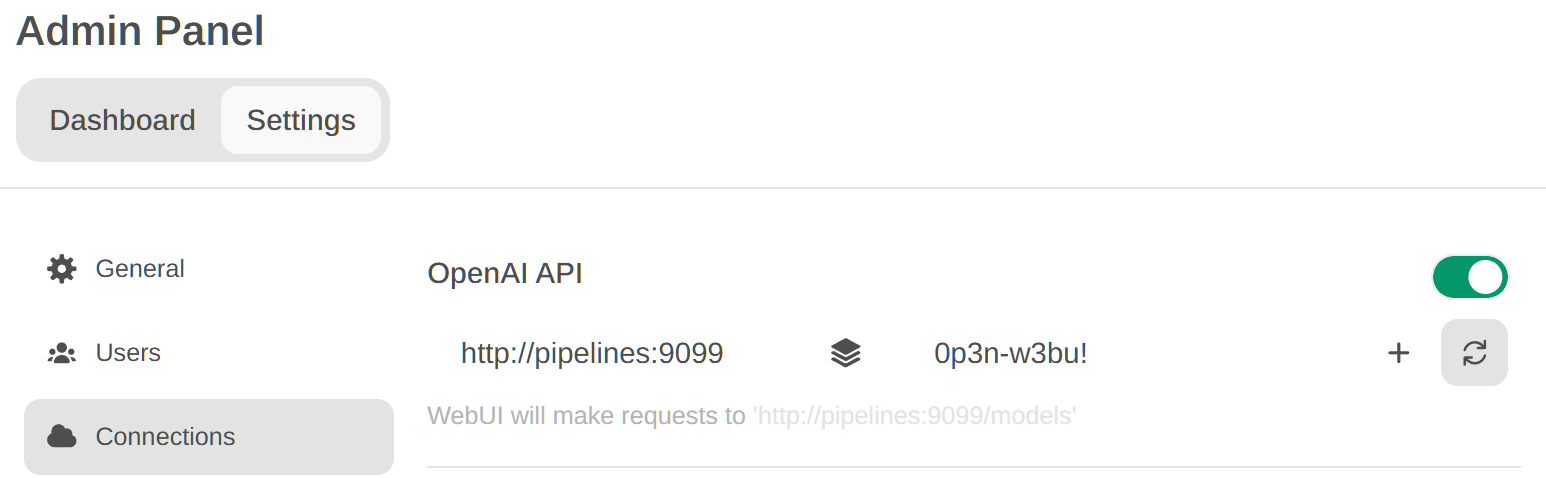
\includegraphics[width=\textwidth,trim=0 0 0 10, clip]{media/openwebui_connections.png}
    \caption{Tela de conexões da OpenWebUI conectando a uma instância do Pipelines. Fonte: autor.\label{fig:openwebui_connections}}
\end{figure*}

\begin{figure}[ht!]
    \centering
    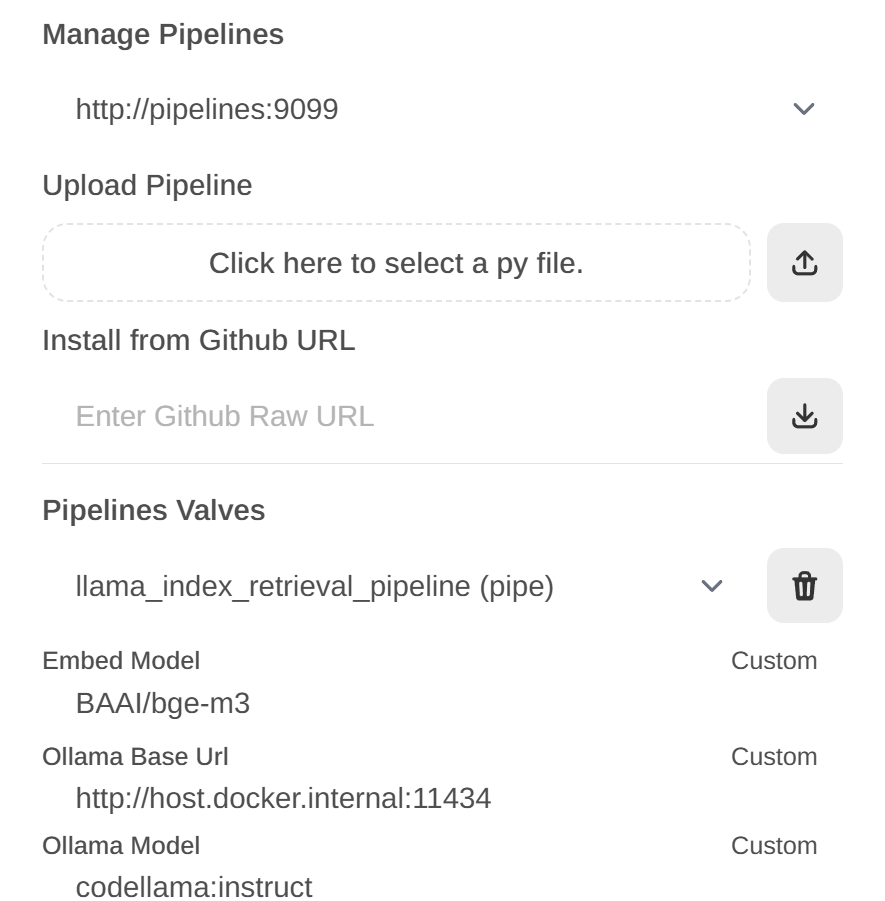
\includegraphics[width=\columnwidth]{media/openwebui_pipeline_config_trim.png}
    \caption{Tela de configuração de uma \textit{pipeline}. Fonte: autor.\label{fig:openwebui_pipeline_config}}
\end{figure}

\section{Implantação em ambiente de produção\label{sec:deploy_prod}}

\noindent%
Nessa seção é apresentado um exemplo de implantação (\textit{deployment}) do sistema completo em produção, que entende-se por um ambiente onde o sistema estará disponível para uso por usuários finais, ou onde o sistema será utilizado de fato.
A \cref{fig:infra_deployment} mostra um diagrama da infraestrutura sugerida para colocar o sistema em uso, não se atentando a detalhes de produtos específicos (marcas e modelos de servidores, roteadores), nem a configurações dos serviços ou da rede.
Itens marcados com um asterisco representam serviços genéricos e em alto nível, onde a escolha de qual empresa ou serviço utilizar fica a critério de quem estiver implementando a arquitetura. 

A configuração do sistema fica sob responsabilidade do implantador.
Dito isso, a grande maioria das configurações necessárias para este projeto são apresentadas na \cref{sec:deploy_test_local}, como endereços de conexão e modelos desejados.
Configurações específicas de serviços externos (\textit{load balancer}, por exemplo) variam muito e, por isso, não são abordadas em detalhes.

Ao analisar a \cref{fig:infra_deployment} observa-se que o sistema é composto por um firewall, uma camada de autenticação, um \textit{load balancer} (LB, balanceador de carga), um \textit{web application firewall} (WAF, um tipo de firewall específico para aplicações web), a Web UI e o modelo.
Dos itens mencionados, o firewall, a camada de autenticação, o \textit{load balancer} e o WAF são serviços genéricos, onde a escolha de qual empresa ou serviço utilizar fica a critério de quem estiver implementando a arquitetura.

\noindent\textbf{Firewall}:
O firewall é responsável por proteger a rede interna de acessos não autorizados e outros ataques a nível de rede.

\noindent\textbf{Autenticação}:
A camada de autenticação é responsável por autenticar os usuários, garantindo que apenas usuários autorizados acessem o sistema.
É sugerido que a autenticação seja feita utilizando o sistema de autenticação único (\textit{single sign-on}, SSO) da instituição, como o Microsoft Entra ID (conhecido também como Microsoft Azure AD) ou o Google Workspace.

\noindent\textbf{\textit{Load balancer}}:
O \textit{load balancer} distribui a carga de requisições entre os servidores, garantindo que nenhum servidor fique sobrecarregado.
Além disso, ele é responsável por fazer a terminação SSL, ou seja, a decodificação do tráfego criptografado, permitindo que o WAF inspecione o tráfego e atue em caso de ataques.

\noindent\textbf{WAF\@}:
O WAF é um tipo de firewall específico para aplicações web que protege a aplicação de ataques direcionados a serviços web como injeção de SQL, \textit{cross-site scripting} (XSS), e mais~\cite{cloudflarewaf}.
Para que o WAF funcione corretamente, é necessário que o tráfego esteja descriptografado, por isso a importância da terminação SSL no \textit{load balancer}.
Após a inspeção do tráfego pelo WAF, ele é encaminhado para o destino original dado pelo \textit{load balancer}.
WAFs modernos atuam como filtros, muitas vezes sendo integrados diretamente ao \textit{load balancer} como um mesmo produto ou serviço.

\noindent\textbf{Web UI\@}:
A Web UI é a interface web do sistema, onde os usuários interagem com o modelo.
Aqui é utilizada a OpenWebUI\@.
A \textit{pipeline} desenvolvida encontra-se nesse mesmo nodo.

\noindent\textbf{Modelo}:
O modelo representa o sistema que está executando o LLM e realizando as tarefas de inferência.
Esse projeto utiliza a ferramenta Ollama.

\begin{figure*}[t!]
    \centering
    \begin{tikzpicture}[%
        % node distance=1em and 1em,
        caption/.style={
            anchor=mid,
            % draw
        },
        diagram item/.style={
            align=center,
            node distance=3.25em,
            % draw
        }]

        \pgfdeclarelayer{background1}
        \pgfdeclarelayer{background2}
        \pgfdeclarelayer{background3}
        \pgfsetlayers{background3,background2,background1,main}

        \node [
            diagram item,
            label=center:Internet
        ] (cloud) {
\includegraphics{cloud}};

        \node [
            diagram item,
            right=1em of cloud,
        ] (fw) {
\includegraphics{firewall}};
        \node[caption] at ([yshift=-0em] fw.north |- cloud.north) {Firewall*};

        \node [
            diagram item,
            right=of fw,
        ] (auth) {
\includegraphics{Network_security}};
        \node[caption] at ([yshift=-0em] auth.north |- cloud.north) {Autenticação*};

        \node [
            diagram item,
            right=of auth,
        ] (lb1) {
\includegraphics{ace}};
        \node[caption] at ([yshift=-0em] lb1.north |- cloud.north) {Load balancer*};

        \node [
            diagram item,
            right=of lb1,
        ] (waf_owui) {
\includegraphics[height=3.75em]{fwsm}};
        \node[caption] (waf_owui_cap) at ([yshift=-0em] waf_owui.north |- cloud.north) {WAF*};

        \node [
            diagram item,
            right=of waf_owui,
        ] (owui) {
\includegraphics{microwebserver}};
        \node[caption] (owui_cap) at ([yshift=-0em] owui.north |- cloud.north) {Web UI};

        \node [
            diagram item,
            right=of owui,
        ] (model) {
\includegraphics{standard_host.pdf}};
        \node[caption] (model_cap) at (model.north |- cloud.north) {Modelo};

        \node[
            diagram item,
            below=of owui,
            shape=circle,
            aspect=2,
            draw
        ] (moodle_plugin) {Plugin} ;

        \node[
            diagram item,
        ] (moodle) at (waf_owui |- moodle_plugin) {
\includegraphics[width=3.5em]{moodlelogo_grayhat_grayscale}};
        \node[caption] at ([xshift=0.2em,yshift=0.25em] moodle.north) {Moodle};

        % Draw arrows
        \draw[thick,-] (cloud) -- (fw) -- (auth) -- (lb1) -- (waf_owui) -- (owui) -- (model);
        \draw[thick,-] ([xshift=-0.3em] moodle_plugin.west) -- (moodle.east);
        \draw[thick,dashed] ([yshift=0.3em] moodle_plugin.north) -- (owui.south);
        \draw[thick,dashed] ([shift={(0.3em,0.3em)}] moodle_plugin.north east) -- (model.south west);

    \end{tikzpicture}
    \caption{%
    Diagrama da possível organização em um ambiente de produção para o sistema apresentado.
    Fonte: autor.\label{fig:infra_deployment}}
\end{figure*}

Por exemplo, os seguintes serviços podem ser utilizados para cada item não-especificado:

\begin{itemize}
    \item Firewall: Fortinet FortiGate-60E.
    \item Autenticação: Microsoft Entra ID integrado à plataforma Cloudflare Zero Trust.
    \item \textit{Load balancer}: HAProxy\footnote{Disponível em:~\url{https://github.com/haproxy/haproxy}} em um servidor dedicado.
    \item WAF\@: Coraza\footnote{Disponível em:~\url{https://github.com/corazawaf/coraza}} no mesmo servidor do HAProxy.
\end{itemize}

Se busca com esse exemplo mostrar que a infraestrutura necessária para colocar o sistema em produção pode ser relativamente simples e de baixo custo operacional.
Ou seja, é possível implantar o sistema em produção sem a necessidade de grandes investimentos em infraestrutura, o que pode ser um fator importante para instituições de ensino com recursos limitados.

De modo geral, o Ollama é o único serviço que precisa estar um servidor dedicado com alto poder de inferência, pois é responsável por executar os modelos de IA\@.
Sendo assim, o servidor que hospeda o Ollama idealmente deve possuir uma GPU de alto desempenho e com ampla memória, como as NVIDIA A100 ou NVIDIA A6000 ou NVIDIA V100, para garantir que os modelos sejam executados de forma eficiente.
O Ollama suporta múltiplas placas de vídeo em um mesmo servidor, o que pode aumentar sua capacidade de inferência;
entretanto, as requisições são atendidads de maneira síncrona, e rodar mais de uma instância do Ollama em um mesmo servidor não é oficialmente suportado.
Se sugere que, caso a demanda seja suficientemente alta, sejam disponibilizados diversos servidores preferencialmente idênticos que executem o Ollama e tenham sua própria placa de vídeo.
A OpenWebUI suporta conexão com múltiplas instâncias do Ollama, distribuindo as requisições entre elas automaticamente.
Outra sugestão é a adoção de sistemas que suportem o paralelismo nativamente como o vLLM, mencionado na~\cref{sec:llm_local}.

Os demais serviços apresentados podem ser executados em máquinas virtuais (Docker, ProxMox\footnote{Disponível em:~\url{https://www.proxmox.com}}), servidores dedicados de baixo custo (microcomputadores ou microprocessadores), ou em serviços de hospedagem na nuvem.

\subsection{Integração com o Moodle}

\noindent%
O Moodle\footnote{Disponível em:~\url{https://moodle.org}} é uma plataforma muito utilizada por instituições de ensino para gerência de materiais de aula e interação com os estudantes.
O Moodle permite a instalação de \textit{plugins} que adicionam funcionalidades à plataforma, o que torna possível a integração do nosso sistema diretamente com a plataforma.
Seria possível integrar tanto a OpenWebUI quanto o modelo com o Moodle, permitindo que os estudantes acessem o sistema diretamente da plataforma, sem a necessidade de acessar um site externo.

Um exemplo de integração é a adição de uma caixa de diálogo na interface do Moodle que permite a interação direta com a \textit{pipeline}, sem a necessidade de redirecionamento.
Como a \textit{pipeline} é uma API que segue a especificação de APIs para inferência da OpenAI, é possível fazer requisições HTTP diretamente para ela, o que facilita essa integração.
Outro exemplo seria a adição de um botão na interface do Moodle que redireciona o usuário para a OpenWebUI, onde ele pode interagir com o sistema normalmente.
As conexões pontilhadas na~\cref{fig:infra_deployment} entre o Moodle, a OpenWebUI e a \textit{pipeline} representam dois dos possíveis métodos de integração já mencionados.

\section{Infraestrutura utilizada\label{sec:infra_nossa}}

\noindent%
A inferência de um LLM é uma tarefa computacionalmente intensiva, e modelos maiores como o LLaMA 3 70B exigem uma quantidade significativa de memória e poder de processamento.
A~\cref{tab:modelos_requisitos} apresenta os requisitos computacionais de alguns LLMs em suas versões \texttt{Instruct}~\cite{ollama}.
Além do requisito de memória, é importante considerar o tempo de inferência, que pode ser significativo para modelos maiores.
Essa medida não foi considerada ao escolher a infraestrutura, pois o tempo de inferência em testes não é um fator crítico.

\begin{table}
    \caption{Requisitos computacionais de LLMs, versões \texttt{Instruct}. Fonte:~\cite{ollama}.\label{tab:modelos_requisitos}}
    \centering
    \begin{tabularx}{\columnwidth}{
        >{\raggedright\arraybackslash}X
        >{\raggedright\arraybackslash}c
        >{\raggedright\arraybackslash}c
        >{\raggedright\arraybackslash}c
    }
        \toprule
        \textbf{Família} & \textbf{Parâmetros} & \textbf{Quantização} & \textbf{Tamanho} \\
        \midrule
        \multirow{5}{*}{LLaMA 3}
        & 8B & Q4\_0 & \SI{4.7}{\giga\byte} \\
        & 8B & FP16 & \SI{16}{\giga\byte} \\
        & 70B & Q4\_0 & \SI{40}{\giga\byte} \\
        & 70B & Q8\_0 & \SI{75}{\giga\byte} \\
        & 70B & FP16 & \SI{141}{\giga\byte} \\
        \midrule
        \multirow{4}{*}{Codellama}
        & 7B  & Q4\_0 & \SI{3.8}{\giga\byte} \\
        & 7B  & FP16 & \SI{13}{\giga\byte} \\
        & 70B & Q4\_0 & \SI{39}{\giga\byte} \\
        & 70B & FP16 & \SI{138}{\giga\byte} \\
        \midrule
        \multirow{4}{*}{Gemma 2}
        & 9B & Q4\_0 & \SI{5.5}{\giga\byte} \\
        & 9B & FP16 & \SI{18}{\giga\byte} \\
        & 27B & Q4\_0 & \SI{16}{\giga\byte} \\
        & 27B & FP16 & \SI{54}{\giga\byte} \\
        \midrule
        \multirow{4}{*}{Mixtral}
        & 8x7B & Q4\_0 & \SI{26}{\giga\byte} \\
        & 8x7B & FP16 & \SI{93}{\giga\byte} \\
        & 8x22B & Q4\_0 & \SI{80}{\giga\byte} \\
        & 8x22B & FP16 & \SI{281}{\giga\byte} \\
        \bottomrule
    \end{tabularx}
\end{table}

Para realizar os testes e treinamentos necessários, foi utilizada uma infraestrutura de servidores dedicados com GPUs NVIDIA A100 de \SI{80}{\giga\byte} de VRAM e NVIDIA RTX 2080 Ti de \SI{11}{\giga\byte} de VRAM, o que permitiu a utilização do modelo LLaMA 3 70B e quantização \SI{8}{\bit}.
Notou-se uma diferença entre os resultados obtidos com modelos quantizados em \SI{8}{\bit} e \SI{4}{\bit}, sendo que o modelo quantizado em \SI{8}{\bit} gerava respostas um pouco mais coerentes.
Esses servidores foram alugados de um provedor de nuvem e configurados com o Ollama e Jupyter Notebooks para execução dos códigos.
Reforça-se novamente a importância de verificar a segurança dos dados ao utilizar serviços de terceiros (\cref{sec:dados_sigilosos}).

\section{Resultados e contribuições\label{sec:resultados}}

\noindent%
Com esse trabalho, espera-se contribuir para o apoio ao aprendizado da programação no ensino superior, auxiliando estudantes a obterem resultados otimizados.
É esperado que o modelo treinado seja capaz de responder perguntas dos estudantes de forma eficiente, eficaz e personalizada, podendo com isso ser utilizado como ferramenta de apoio ao aprendizado.

Este trabalho fornece uma ferramenta que gera dados para análise de aprendizado (\textit{learning analytics}), podendo levar a mudanças nos objetos de aprendizagem e metodologias de aprendizagem utilizadas pelo professor.
Por exemplo, o sistema pode fornecer informações (\textit{insights}) sobre as principais dúvidas dos estudantes, os tópicos mais difíceis de serem compreendidos, entre outros, indicando até mesmo a necessidade de mudanças no currículo ou na abordagem de ensino.

\subsection{Resultados obtidos}

\noindent%
Os resultados obtidos com a implantação do sistema em ambiente de teste foram satisfatórios.
O sistema foi capaz de responder perguntas de forma coerente e correta, fornecendo informações úteis e relevantes dado um contexto.

Por mais que não tenham sido conduzidos testes do sistema desenvolvido com alunos de uma turma da disciplina de Fundamentos da Programação, a metodologia de testes e perguntas utilizadas baseou-se em perguntas reais desses alunos.

A~\cref{fig:exemplo_interacao} apresenta um exemplo de interação entre um usuário intencionalmente vago e impreciso, e o LLM\@.
O usuário está sendo propositalmente vago para avaliar a capacidade do assistente de inferir o contexto e fornecer uma resposta adequada.
Essa interação se deu através da OpenWebUI e fora convertida para Markdown pois não foi possível englobar toda a conversa em uma imagem só.
O usuário não dá muitos detalhes sobre o problema, mas o assistente foi capaz de inferir o contexto e fornecer uma resposta adequada, guiando o usuário para a solução do problema.
O exemplo que o assistente deu ao falar sobre a estrutura do \texttt{for} em Java foi citada diretamente dos materiais fornecidos pelo RAG, demonstrando que ele foi capaz de absorver e aplicar o conhecimento fornecido.

\begin{figure*}[h]
    \centering
    \begin{minted}{markdown}
# User
meu programa não tá funcionando

# Assistant
Não funciona, é? Vamos tentar descobrir o que pode estar acontecendo.
Você escreveu o programa usando uma linguagem de programação, certo?
Pode me mostrar o código do seu programa? Isso vai me ajudar a entender melhor o que pode estar acontecendo.
Além disso, você já tentou executar o programa passo a passo para ver onde ele está falhando?
Você está usando algum tipo de loop no seu programa, como o exemplo que vimos na aula de repetição?
Deseja mais detalhes sobre como depurar um programa ou como usar loops de repetição?

# User
for i 0 .. 10 i++
imprime(i)

# Assistant
Você está tentando escrever um loop for para imprimir os números de 0 a 10!
No entanto, parece que há alguns erros de sintaxe no seu código. Vamos corrigir isso juntos!
Em Java, o loop for é escrito da seguinte maneira:
```java
for (inicialização; condição; incremento) {
  // bloco de código
}
```
No seu caso, você pode escrever o loop for como:
```java
for (int i = 0; i <= 10; i++) {
  System.out.println(i);
}
```
Observe que:
- int i = 0 é a inicialização do loop, onde você define a variável i com valor inicial 0.
- i <= 10 é a condição do loop, que verifica se i é menor ou igual a 10.
- i++ é o incremento do loop, que aumenta o valor de i em 1 a cada iteração.
- System.out.println(i) é o bloco de código que imprime o valor de i na tela.
Tente executar esse código e veja se ele funciona como esperado!
Deseja mais detalhes sobre como funciona o loop for ou como imprimir valores na tela em Java?
    \end{minted}
    \caption{%
    Exemplo de interação entre o usuário e o assistente virtual. Fonte: autor.\label{fig:exemplo_interacao}}
\end{figure*}

Um resultado impressionante foi o seguinte, que, ao ser perguntado ``O que é uma rede neural?\,'', o modelo respondeu o seguinte:

\begin{quote}{LLaMA 3, \textit{Pipeline}}
Uma rede neural! Isso é um tópico interessante em inteligência artificial. Embora não esteja diretamente relacionado ao conteúdo de linguagem algorítmica e programação que estamos estudando, posso dar uma visão geral sobre o que é uma rede neural.

Uma rede neural é um modelo de processamento de informações inspirado no funcionamento do cérebro humano. É composta por uma série de camadas de neurônios artificiais que se comunicam entre si, processando e transmitindo informações.

Imagine uma rede de neurônios que se conectam e se comunicam entre si, permitindo que a informação flua e seja processada de forma complexa. Isso permite que as redes neurais aprendam e sejam treinadas para realizar tarefas como reconhecimento de padrões, classificação de dados e tomada de decisões.

No entanto, para entender melhor como as redes neurais funcionam, precisamos voltar ao básico e estudar como os algoritmos e a programação são utilizados para criar essas redes.

Você gostaria de saber mais sobre como os algoritmos são utilizados para criar redes neurais? Ou gostaria de voltar ao conteúdo de linguagem algorítmica e programação que estamos estudando?
\end{quote}

A relação que o modelo fez entre redes neurais e o conteúdo da disciplina não está em nenhum dos materiais passados a ele.
Além disso, ele deu uma boa explicação sobre redes neurais, mesmo que em alto nível, própria para iniciantes.
Somado a isso, reforçou a importância de estudar os básicos e se dispôs a apoiar o usuário.

De modo geral, o sistema atende as expectativas do ponto de vista de um discente com dúvidas.
Além disso, como demonstrado na~\cref{sec:learning_analytics}, o sistema traz ferramentas de suporte ao trabalho do docente.

\subsection{Problemas enfrentados}

\noindent%
Durante o desenvolvimento e testes do sistema, alguns problemas foram encontrados e resolvidos.
Em um dos testes iniciais, demonstrado na~\cref{fig:corolla}, ao ser questionado que tipo de modelo ele é, o modelo respondeu ``Corolla'', um tipo de carro.
Em outro, ao testar se o modelo mantinha o contexto, ele começou a falar em inglês; ao ser instruído a falar português, ele começou a misturar ambas as línguas.
Similar à situação anterior, após mencionar algum termo em inglês como \textit{for} ou \textit{loop}, o modelo gerava o restante da resposta em inglês.
Possivelmente, essa preferência por inglês é resultado do processo de treino do LLaMA 3, que utilizou um \textit{dataset} majoritariamente em inglês.

\begin{figure}[h]
    \centering
    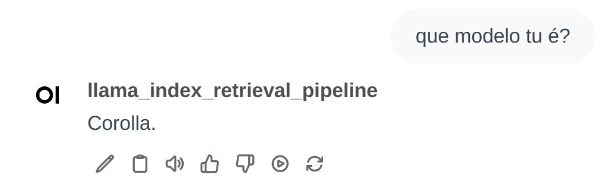
\includegraphics[width=\columnwidth]{media/corolla.png}
    \caption{%
    Exemplo de resposta inesperada do modelo. Fonte: autor.\label{fig:corolla}}
\end{figure}

Além de empecilhos referentes ao uso de IA, foram encontrados diversas outras situações ao longo do desenvolvimento do projeto.
Uma delas foi a grande quantidade de maneiras de abordar um mesmo problema ou situação; muitas vezes se encontraram soluções diferentes que traziam o mesmo resultado.
Por exemplo, a biblioteca LlamaIndex apresenta ao menos três maneiras diferentes de se carregar um arquivo e ao menos sete maneiras diferentes de interagir com esses dados.
Levando em consideração que existem dezenas de outras bibliotecas de RAG disponíveis, a quantidade de documentação existente é imensa.

Outros problemas foram os de implementação da \textit{pipeline}.
O \textit{framework} Pipelines é extremamente novo, publicado em Maio de 2024, fato que provavelmente explica a falta de documentação disponível, o que tornou necessária, em vezes, a leitura do código-fonte para atingir algum determinado objetivo não-documentado.
A situação mais grave encontrada até o momento foi que, ao utilizar o motor de \textit{chat} do \texttt{LlamaIndex}, todos os usuários compartilhavam um mesmo histórico de conversa.
Ou seja, caso o usuário Alice estivesse conversando sobre laços e o usuário Bob entrasse no sistema e perguntasse ``Qual a mensagem anterior?\,'' em uma nova conversa em sua própria conta, o sistema retornava a Bob a última mensagem que trocou com Alice.
Um problema gravíssimo, tanto de coerência quanto de privacidade.
Para corrigir essa situação, modificou-se o código da \textit{pipeline} para que apenas o histórico daquele usuário fosse repassado ao modelo.
A~\cref{fig:convert_history_to_chat_history} apresenta a correção, onde \mintinline{python}|self| refere-se à classe da \textit{pipeline}.

\begin{figure}
    \centering
    \begin{minted}[python3,highlightlines={10-12}]{python}
def pipe(
  self,
  user_message: str,
  model_id: str,
  messages: list[dict],
  body: dict,
) -> Union[str, Generator, Iterator]:
  response = self.engine.stream_chat(
    user_message,
    chat_history=self.dict_to_chatmessages(
      messages
    )
  )
  return response.response_gen

@staticmethod
def dict_to_chatmessages(
    messages: list[dict[str, str]]
) -> list[ChatMessage]:
  return [
    ChatMessage(**msg) for msg in messages
  ]
    \end{minted}
    \caption{Código de correção do compartilhamento de histórico entre todos os usuários.
    As linhas demarcadas (10--12) e a função \mintinline{python}|dict_to_chatmessages| são a correção.\label{fig:convert_history_to_chat_history}}
\end{figure}

\section{Limitações\label{sec:limitacoes}}

\noindent%
O sistema apresentado possui algumas limitações, tanto de escopo quanto de implementação.

\subsection{Limitações de escopo}

\noindent%
O estudo se limitou a um único LLM, utilizando apenas um sistema para rodá-lo (Ollama), com forte integração com a OpenWebUI e ao Pipelines.
Além disso, os dados utilizados para munir o sistema de conhecimento são focados em apenas uma disciplina de programação, com um professor, em apenas uma universidade, ao longo de um semestre.

\subsection{Limitações técnicas}

\noindent%
Limitações técnicas também são encontradas, como a \ul{necessidade de um servidor computacionalmente potente} --- em outras palavras, de alto custo --- para executar um LLM de maior capacidade de inferência.

A maioria dos LLMs atuais são treinados em \textit{corpus} textuais primariamente compostos por conteúdos em inglês.
Como mencionado na~\cref{sec:llama3}, o LLaMA 3 não é diferente: fora treinado em um \textit{dataset} com $15$ trilhões de \textit{tokens}, sendo que apenas $5\%$ desse conjunto são de línguas diferentes do inglês, uma quantidade significativamente menor de dados.
Logo, a performance dos modelos em outras línguas, por dedução, é menor do que sua performance quando infere em sua língua-mãe.
Essa mesma limitação se aplicou ao modelo de \textit{embedding}, como mencionado na~\cref{sec:escolha_embedding}.
Ao dizer ``performance'', pode-se interpretar como problemas de acurácia, limitações de interpretação de contexto e \textit{bias} do \textit{dataset}.
Para mitigar essa limitação, se sugerem algumas estratégias:

\begin{itemize}
    \item \textit{Fine-tuning} do modelo em um \textit{dataset} com mais dados em português.
    \item Adicionar sistemas de tradução antes e depois do modelo, como numa \textit{pipeline}, para que o modelo sempre execute em sua melhor língua.
\end{itemize}

\section{Considerações finais\label{sec:conclusao}}

\noindent%
Este estudo explorou o uso de Inteligência Artificial Generativa como uma ferramenta de apoio ao aprendizado de programação, com o objetivo de investigar seus potenciais benefícios e limitações.
A pesquisa apresentou um sistema que integra materiais didáticos à IA, potencialmente promovendo ambientes personalizados de aprendizagem capazes de coletar informações valiosas para análise do aprendizado.
Também foi apresentada uma arquitetura de implantação do sistema em ambiente de produção, com sugestões de serviços e configurações.

Os resultados obtidos, a despeito das limitações indicadas, demonstraram que a implementação de IA Generativa pode fornecer suporte personalizado aos estudantes, e acredita-se que possa ajudá-los a superar obstáculos de aprendizagem de maneira individualizada.
O sistema foi capaz de responder perguntas de forma eficiente e satisfatória, proporcionando \textit{feedback} em tempo real e exemplos de código contextualizados, alinhando-se com os materiais de apoio utilizados nas disciplinas.

Apesar dos benefícios observados, foi identificado, durante o processo de desenvolvimento deste texto por este autor, algumas limitações, como a necessidade de servidores computacionalmente potentes para executar os LLMs, o que implica em altos custos, o que pode dificultar a adoção desse sistema por instituições com recursos limitados.

Em termos de impacto, espera-se que a adoção de sistemas de IA Generativa no aprendizado de programação possa contribuir de alguma forma para dar suporte ao trabalho do professor.
No entanto, este texto também reforça a importância de docentes e ferramentas de IA trabalharem juntos, assim como a necessidade de treinamentos e capacitações para que os professores possam utilizar essas ferramentas de forma eficaz.
A ferramenta também visa oferecer informações que facilitem o trabalho dos docentes, podendo identificar padrões de aprendizado e áreas de dificuldade dos alunos.

Em suma, acredita-se que este trabalho contribui para a área de IA como apoio ao aprendizado, demonstrando que a integração de tecnologias avançadas no aprendizado de programação tem potencial para tornar o aprendizado mais acessível, intuitivo e eficiente, beneficiando tanto alunos quanto instituições de ensino.

\section{Trabalhos futuros\label{sec:trabs_futuros}}

\noindent%
Este estudo apresentou um sistema pensado para ser modular e de fácil expansão.
Áreas de interesse para trabalhos futuros:

\begin{itemize}
    \item Treinar um modelo em um \textit{dataset} com mais dados em português.
    \item Testar modelos diferentes de \textit{embedding}.
    \item Adicionar à \textit{pipeline} sistemas de instrumentação automatizados que recolham dados e \textit{logs} das conversas para fim de aplicar técnicas de análise do aprendizado.
    \item Verificar a performance do sistema com um \textit{dataset} maior.
    \item Implementar um RAG multi-agente onde cada agente possui um nível incremental de conhecimento $n_{i} = n_{i-1} + 1$.
    Essa abordagem pode ser útil quando se deseja limitar o conhecimento de um modelo à uma sequência incremental de dados.
    Por exemplo, cada agente estaria ciente da matéria até certo ponto, podendo haver a troca de agentes conforme o usuário avança no currículo.
    \item Adicionar informações sobre o usuário ao sistema como arquivos de provas passadas, trabalhos e notas para personalizar a experiência de modo individual.
    \item Disponibilizar para grupos de usuários ao longo de um ou mais semestres para identificar outras potencialidades ou limitações.
\end{itemize}

% todo verificar citações e remover \nocite
% \nocite{*}
\bibliographystyle{IEEEtran}
\bibliography{ref}

\section*{Uso de Inteligência Artificial}
\noindent%
Este trabalho utilizou Inteligência Artificial (IA) para correção de textos.

\begin{IEEEbiographynophoto}{Rafael Almeida de Bem}
Aluno de Ciência da Computação na Pontifícia Universidade Católica do Rio Grande do Sul (PUCRS).
Possui interesse em Inteligência Artificial e Aprendizado de Máquina.
Tem experiência em desenvolvimento de software \textit{back-end}, manutenção de infraestrutura e automação de processos.
\end{IEEEbiographynophoto}

\end{document}
